\documentclass[11pt,a4paper,oneside]{report}
\usepackage[T1]{fontenc}
\usepackage[utf8]{inputenc}
\usepackage[italian]{babel}
\usepackage{amsmath,amssymb}
\usepackage{mathtools}
\usepackage{siunitx}
\usepackage{graphicx}
\usepackage{booktabs}
\usepackage{longtable}
\usepackage{array}
\usepackage{geometry}
\usepackage{hyperref}
\usepackage{xcolor}
\usepackage{float}
\usepackage{tikz}
\usepackage{listings}
\lstset{language=Matlab,basicstyle=\ttfamily\footnotesize,
  columns=fullflexible,keepspaces=true,breaklines=true,
  showstringspaces=false,tabsize=2,frame=single,
  rulecolor=\color{black!20},commentstyle=\color{black!60},
  keywordstyle=\color{blue!45!black},aboveskip=.7em,belowskip=.7em}
\usepackage[protrusion=true,expansion=false]{microtype}
\geometry{top=2.5cm,bottom=2.5cm,left=2.7cm,right=2.3cm}
\hypersetup{hypertexnames=false,colorlinks=true,linkcolor=blue!45!black,urlcolor=blue!55!black,pdftitle={Controllo robusto di un manipolatore planare 2-DoF con SEA},pdfauthor={Alessio de Dato; Valerio Rebechi}}
\setlength{\emergencystretch}{3em}
\setlength{\parindent}{1.2em}
\renewcommand{\arraystretch}{1.12}
\newcommand{\status}[1]{\texttt{#1}}
\newcommand{\artifact}[1]{\texttt{#1}}
\newcommand{\FinResiduoEquilibrio}{\num{5.84e-14}}
\newcommand{\FinErroreJacobiano}{\num{6.17e-11}}
\newcommand{\FinErroreAB}{\num{1.32e-14}}
\newcommand{\FinErroreLFT}{\num{0}}
\newcommand{\FinCopertura}{\num{0.9801}}
\newcommand{\FinHoldout}{\num{0.9436}}
\newcommand{\FinPesoFormula}{\frac{1049s+0.009319}{s^{3}+137.2s^{2}+5241s+1.022\cdot10^{5}}}
\newcommand{\FinCARELQG}{\num{4.34e-13}}
\newcommand{\FinCARELQGI}{\num{3.49e-13}}
\newcommand{\FinScartoMixsyn}{\num{3.12e-12}}
\newcommand{\FinOrdinePeso}{3}
\newcommand{\FinGammaMix}{\num{0.953412}}
\newcommand{\FinGammaPID}{\num{0.831584}}
\newcommand{\FinSeparazione}{\num{1.75e-13}}
\newcommand{\FinDkA}{\num{2.929}}
\newcommand{\FinDkB}{\num{1.811}}
\newcommand{\FinOccorrenze}{17}
\newcommand{\FinAlphaLqr}{\num{6.219}}
\newcommand{\FinAlphaKalman}{\num{9.319}}
\newcommand{\FinRapportoKalman}{\num{1.499}}
\newcommand{\FinLQGStable}{10}
\newcommand{\FinLQGConv}{15}
\newcommand{\FinLQGPeak}{\num{0.415}}
\newcommand{\FinLQGRms}{\num{0.0809}}
\newcommand{\FinLQGTs}{\num{0.671}}
\newcommand{\FinLQGEss}{0}
\newcommand{\FinLQGMp}{\num{0.411}}
\newcommand{\FinLQGCross}{\num{17}}
\newcommand{\FinLQGTrackPeak}{\num{4.75}}
\newcommand{\FinLQGTarget}{PASS}
\newcommand{\FinLQGNonConv}{0}
\newcommand{\FinLQGDiv}{0}
\newcommand{\FinLQGRSA}{\num{1.454}}
\newcommand{\FinLQGRSesitoA}{PASS}
\newcommand{\FinLQGRPesitoA}{FAIL}
\newcommand{\FinLQGNorma}{\num{2.168}}
\newcommand{\FinLQGOrdine}{14}
\newcommand{\FinLQGOrdineChiuso}{28}
\newcommand{\FinLQGIntervalloRSA}{[\num{1.454}, \num{1.505}]}
\newcommand{\FinLQGFrequenzaA}{\num{57.56}}
\newcommand{\FinLQGRSB}{\num{1.195}}
\newcommand{\FinLQGRSesitoB}{PASS}
\newcommand{\FinLQGRPesitoB}{FAIL}
\newcommand{\FinLQGIntervalloRSB}{[\num{1.195}, \num{1.197}]}
\newcommand{\FinLQGFrequenzaB}{\num{42.8}}
\newcommand{\FinLQGIStable}{10}
\newcommand{\FinLQGIConv}{15}
\newcommand{\FinLQGIPeak}{\num{0.43}}
\newcommand{\FinLQGIRms}{\num{0.0839}}
\newcommand{\FinLQGITs}{\num{5.05}}
\newcommand{\FinLQGIEss}{0}
\newcommand{\FinLQGIMp}{\num{0}}
\newcommand{\FinLQGICross}{\num{3.6}}
\newcommand{\FinLQGITrackPeak}{\num{0.822}}
\newcommand{\FinLQGITarget}{FAIL}
\newcommand{\FinLQGINonConv}{0}
\newcommand{\FinLQGIDiv}{0}
\newcommand{\FinLQGIRSA}{\num{1.406}}
\newcommand{\FinLQGIRSesitoA}{PASS}
\newcommand{\FinLQGIRPesitoA}{FAIL}
\newcommand{\FinLQGINorma}{\num{1.261}}
\newcommand{\FinLQGIOrdine}{16}
\newcommand{\FinLQGIOrdineChiuso}{30}
\newcommand{\FinLQGIIntervalloRSA}{[\num{1.406}, \num{1.455}]}
\newcommand{\FinLQGIFrequenzaA}{\num{57.86}}
\newcommand{\FinLQGIRSB}{\num{1.152}}
\newcommand{\FinLQGIRSesitoB}{PASS}
\newcommand{\FinLQGIRPesitoB}{FAIL}
\newcommand{\FinLQGIIntervalloRSB}{[\num{1.152}, \num{1.155}]}
\newcommand{\FinLQGIFrequenzaB}{\num{42.74}}
\newcommand{\FinHinfOneStable}{10}
\newcommand{\FinHinfOneConv}{15}
\newcommand{\FinHinfOnePeak}{\num{0.299}}
\newcommand{\FinHinfOneRms}{\num{0.058}}
\newcommand{\FinHinfOneTs}{\num{1.53}}
\newcommand{\FinHinfOneEss}{\num{14.2}}
\newcommand{\FinHinfOneMp}{\num{125}}
\newcommand{\FinHinfOneCross}{\num{38}}
\newcommand{\FinHinfOneTrackPeak}{\num{14}}
\newcommand{\FinHinfOneTarget}{FAIL}
\newcommand{\FinHinfOneNonConv}{0}
\newcommand{\FinHinfOneDiv}{0}
\newcommand{\FinHinfOneRSA}{\num{1.407}}
\newcommand{\FinHinfOneRSesitoA}{PASS}
\newcommand{\FinHinfOneRPesitoA}{FAIL}
\newcommand{\FinHinfOneNorma}{\num{2.131}}
\newcommand{\FinHinfOneOrdine}{18}
\newcommand{\FinHinfOneOrdineChiuso}{32}
\newcommand{\FinHinfOneIntervalloRSA}{[\num{1.407}, \num{1.424}]}
\newcommand{\FinHinfOneFrequenzaA}{\num{78.84}}
\newcommand{\FinHinfOneRSB}{\num{1.014}}
\newcommand{\FinHinfOneRSesitoB}{PASS}
\newcommand{\FinHinfOneRPesitoB}{FAIL}
\newcommand{\FinHinfOneIntervalloRSB}{[\num{1.014}, \num{1.018}]}
\newcommand{\FinHinfOneFrequenzaB}{\num{78.99}}
\newcommand{\FinHinfTwoStable}{1}
\newcommand{\FinHinfTwoConv}{13}
\newcommand{\FinHinfTwoPeak}{\num{3.67e+05}}
\newcommand{\FinHinfTwoRms}{\num{1.07e+04}}
\newcommand{\FinHinfTwoTs}{\num{1.94}}
\newcommand{\FinHinfTwoEss}{\num{0.106}}
\newcommand{\FinHinfTwoMp}{\num{0}}
\newcommand{\FinHinfTwoCross}{\num{0.855}}
\newcommand{\FinHinfTwoTrackPeak}{\num{0.821}}
\newcommand{\FinHinfTwoTarget}{PASS}
\newcommand{\FinHinfTwoNonConv}{0}
\newcommand{\FinHinfTwoDiv}{2}
\newcommand{\FinHinfTwoRSA}{\num{0.04399}}
\newcommand{\FinHinfTwoRSesitoA}{FAIL}
\newcommand{\FinHinfTwoRPesitoA}{FAIL}
\newcommand{\FinHinfTwoNorma}{\num{0.0312}}
\newcommand{\FinHinfTwoOrdine}{22}
\newcommand{\FinHinfTwoOrdineChiuso}{36}
\newcommand{\FinHinfTwoIntervalloRSA}{[\num{0.04399}, \num{0.04767}]}
\newcommand{\FinHinfTwoFrequenzaA}{\num{62.73}}
\newcommand{\FinHinfTwoRSB}{\num{0.04025}}
\newcommand{\FinHinfTwoRSesitoB}{FAIL}
\newcommand{\FinHinfTwoRPesitoB}{FAIL}
\newcommand{\FinHinfTwoIntervalloRSB}{[\num{0.04025}, \num{0.04033}]}
\newcommand{\FinHinfTwoFrequenzaB}{\num{62.74}}
\newcommand{\FinPIDStable}{8}
\newcommand{\FinPIDConv}{0}
\newcommand{\FinPIDPeak}{\num{1.07e+03}}
\newcommand{\FinPIDRms}{\num{14.2}}
\newcommand{\FinPIDTs}{\num{3.7}}
\newcommand{\FinPIDEss}{0}
\newcommand{\FinPIDMp}{\num{2.48}}
\newcommand{\FinPIDCross}{\num{50.5}}
\newcommand{\FinPIDTrackPeak}{\num{4.02}}
\newcommand{\FinPIDTarget}{FAIL}
\newcommand{\FinPIDNonConv}{15}
\newcommand{\FinPIDDiv}{0}
\newcommand{\FinPIDRSA}{\num{0.231}}
\newcommand{\FinPIDRSesitoA}{FAIL}
\newcommand{\FinPIDRPesitoA}{FAIL}
\newcommand{\FinPIDNorma}{\num{0.8298}}
\newcommand{\FinPIDOrdine}{4}
\newcommand{\FinPIDOrdineChiuso}{18}
\newcommand{\FinPIDIntervalloRSA}{[\num{0.231}, \num{0.2345}]}
\newcommand{\FinPIDFrequenzaA}{\num{18.54}}
\newcommand{\FinPIDRSB}{\num{0.1702}}
\newcommand{\FinPIDRSesitoB}{FAIL}
\newcommand{\FinPIDRPesitoB}{FAIL}
\newcommand{\FinPIDIntervalloRSB}{[\num{0.1702}, \num{0.171}]}
\newcommand{\FinPIDFrequenzaB}{\num{18.54}}
\newcommand{\FinMuAStable}{10}
\newcommand{\FinMuAConv}{15}
\newcommand{\FinMuAPeak}{\num{459}}
\newcommand{\FinMuARms}{\num{47.5}}
\newcommand{\FinMuATs}{\num{5.13}}
\newcommand{\FinMuAEss}{\num{28}}
\newcommand{\FinMuAMp}{\num{0}}
\newcommand{\FinMuACross}{\num{4.38}}
\newcommand{\FinMuATrackPeak}{\num{0.612}}
\newcommand{\FinMuATarget}{FAIL}
\newcommand{\FinMuANonConv}{0}
\newcommand{\FinMuADiv}{0}
\newcommand{\FinMuARSA}{\num{2.662}}
\newcommand{\FinMuARSesitoA}{PASS}
\newcommand{\FinMuARPesitoA}{FAIL}
\newcommand{\FinMuANorma}{\num{1.895}}
\newcommand{\FinMuAOrdine}{242}
\newcommand{\FinMuAOrdineChiuso}{256}
\newcommand{\FinMuAIntervalloRSA}{[\num{2.662}, \num{3.447}]}
\newcommand{\FinMuAFrequenzaA}{\num{15.22}}
\newcommand{\FinMuARSB}{\num{1.956}}
\newcommand{\FinMuARSesitoB}{PASS}
\newcommand{\FinMuARPesitoB}{FAIL}
\newcommand{\FinMuAIntervalloRSB}{[\num{1.956}, \num{1.96}]}
\newcommand{\FinMuAFrequenzaB}{\num{23.01}}
\newcommand{\FinMuBStable}{10}
\newcommand{\FinMuBConv}{15}
\newcommand{\FinMuBPeak}{\num{574}}
\newcommand{\FinMuBRms}{\num{36.5}}
\newcommand{\FinMuBTs}{\num{3.4}}
\newcommand{\FinMuBEss}{\num{14.8}}
\newcommand{\FinMuBMp}{\num{0}}
\newcommand{\FinMuBCross}{\num{3.68}}
\newcommand{\FinMuBTrackPeak}{\num{0.8}}
\newcommand{\FinMuBTarget}{FAIL}
\newcommand{\FinMuBNonConv}{0}
\newcommand{\FinMuBDiv}{0}
\newcommand{\FinMuBRSA}{\num{2.469}}
\newcommand{\FinMuBRSesitoA}{PASS}
\newcommand{\FinMuBRPesitoA}{FAIL}
\newcommand{\FinMuBNorma}{\num{1.087}}
\newcommand{\FinMuBOrdine}{106}
\newcommand{\FinMuBOrdineChiuso}{120}
\newcommand{\FinMuBIntervalloRSA}{[\num{2.469}, \num{2.549}]}
\newcommand{\FinMuBFrequenzaA}{\num{65.81}}
\newcommand{\FinMuBRSB}{\num{1.825}}
\newcommand{\FinMuBRSesitoB}{PASS}
\newcommand{\FinMuBRPesitoB}{FAIL}
\newcommand{\FinMuBIntervalloRSB}{[\num{1.825}, \num{1.829}]}
\newcommand{\FinMuBFrequenzaB}{\num{32.42}}

\hypersetup{pdftitle={Capitolo 7 - LQG e LQGI - intervento pilota}}
\begin{document}
\tableofcontents
\clearpage
\setcounter{chapter}{6}
\chapter{Controllo LQG}
\section{Obiettivo e architettura}
Il regolatore usa il modello nominale M3 a 14 stati e le quattro misure encoder
$y=[\Delta q^T,\Delta\theta^T]^T$. Le velocità e gli stati interni degli attuatori
non sono misurati. LQR progetta il feedback supponendo lo stato disponibile;
Kalman lo ricostruisce da modello, ingressi e misure. La legge effettivamente
implementata è $u=-K\hat x+N_rr$, nelle coordinate incrementali M2.
Il prefiltro rende unitario il guadagno statico nominale riferimento--posizione,
ma non contiene un modello interno dei disturbi costanti.

\section{Scelta e normalizzazione di Q e R}
\subsection{Il problema LQR e le unità fisiche}
Il costo è
\[
J=\int_0^\infty \left(x^TQx+u^TRu\right)\,dt .
\]
Il primo termine penalizza gli scostamenti delle coordinate fisiche di interesse;
il secondo penalizza le coppie di comando. Il compromesso fra transitorio e
sforzo dipende da entrambi. Usare una matrice identità senza spiegazione
assegnerebbe lo stesso coefficiente numerico a radianti, radianti al secondo e
coordinate arbitrarie di realizzazione, senza renderne comparabili gli effetti.

Lo stato completo, in deviazione dall'equilibrio, è
\[
x=[\Delta q_1,\Delta q_2,\Delta\dot q_1,\Delta\dot q_2,
\Delta\theta_1,\Delta\theta_2,\Delta\dot\theta_1,\Delta\dot\theta_2,x_a^T]^T.
\]
I sei elementi di $x_a$ appartengono alla realizzazione \texttt{ss} dei due
attuatori secondo ordine--Padé; le loro unità dipendono dalla realizzazione,
non sono ulteriori posizioni fisiche. Non viene attribuita loro una scala
meccanica inventata e non ricevono una penalizzazione diretta. Restano comunque
nel modello, nel feedback e nella verifica di stabilità.

\subsection{Scale e provenienza: il significato esatto di qs}
Distinguiamo parametri imposti dalla traccia (A), derivati matematicamente (B),
ricavati da grandezze fisiche (C), scelti nel progetto (D) e selezionati dalla
ricerca (E). Questa distinzione evita di attribuire al docente scelte nostre.

\begin{table}[H]\centering\small
\begin{tabular}{p{3.4cm}p{3.5cm}p{6.6cm}}\toprule
Grandezza del costo & Scala & Origine e significato\\\midrule
$\Delta q_i$ [rad] & $q_s=5\pi/180$ & C da M5-D: ampiezza del riferimento nominale.\\
$\Delta\dot q_i$ [rad/s] & $\dot q_s=12q_s$ & C: velocità caratteristica banda per ampiezza; non velocità massima.\\
$\Delta\theta_i-\Delta q_i$ [rad] & $\delta_s=0.5/40=0.0125$ & C da coppia di disturbo M5-D e rigidezza minima della traccia-A. Scala comune della molla più cedevole.\\
$\Delta\dot\theta_i$ [rad/s] & $\dot\theta_s=\dot q_s$ & D/C: stessa scala cinematica scelta per i motori; non un vincolo.\\
$x_a$ (6 coordinate) & nessuna scala diretta & Nessuna penalizzazione diretta di coordinate dipendenti dalla realizzazione.\\
\bottomrule\end{tabular}
\caption{Scale del costo M6: derivazioni fisiche basate su scelte M5, non nuovi limiti hardware.}
\end{table}

Nel codice di produzione \path{build_lqr_state_cost.m} l'assegnazione è:
\begin{verbatim}
scales.q = m5Spec.referenceAmplitude;
\end{verbatim}
Nel file didattico la medesima
grandezza è chiamata \texttt{qs} e definita nella sezione 5.
Quindi $q_s=\RevQs$ rad è una \emph{scala dimensionale}, non un peso relativo,
non un candidato di tuning e non un risultato della ricerca.
Il peso adimensionale sulla posizione si chiama invece $w_q$.
La scala di velocità effettiva è \RevQds\ rad/s; quella di deformazione
è \RevDeltaScale\ rad. $\Delta\theta$ non viene pesata isolatamente:
entra attraverso la deformazione $\Delta\theta-\Delta q$.

\subsection{Trasformazione esplicita e matrice Q non diagonale}
Introduciamo le otto uscite fisiche del costo:
\[
v=Fx=\begin{bmatrix}\Delta q\\\Delta\dot q\\
\Delta\theta-\Delta q\\\Delta\dot\theta\end{bmatrix},\qquad
F=\begin{bmatrix}
I_2&0&0&0&0\\0&I_2&0&0&0\\-I_2&0&I_2&0&0\\0&0&0&I_2&0
\end{bmatrix}.
\]
L'ultima colonna a blocchi ha sei colonne scalari. Le posizioni sono quindi
penalizzate sia come errore articolare sia come parte della deformazione.
Definiamo
\[
S_x=\operatorname{diag}(q_sI_2,\dot q_sI_2,\delta_sI_2,\dot\theta_sI_2),
\quad \tilde v=S_x^{-1}Fx,\quad
W_q=\operatorname{diag}(w_qI_2,w_vI_2,w_\delta I_2,w_vI_2).
\]
Qui $S_x$ è $8\times8$ perché normalizza le uscite del costo, non uno stato
trasformato invertibile di dimensione 14. Ne segue esattamente
\[
x^TQx=\tilde v^TW_q\tilde v,\qquad
Q=F^TS_x^{-T}W_qS_x^{-1}F=C_{cost}^TC_{cost},\quad
C_{cost}=W_q^{1/2}S_x^{-1}F.
\]
Per ogni uscita normalizzata il coefficiente è $w_i/s_i^2$.
Espandendo il termine elastico compaiono coefficienti incrociati negativi fra
$q_i$ e $\theta_i$. Pertanto scrivere semplicemente $Q=\operatorname{diag}(q_i)$
sarebbe errato per questo progetto. $Q$ è semidefinita positiva: il blocco
attuativo nullo non implica assenza degli attuatori dalla dinamica ottimizzata.

\subsection{R: scala di comando e peso di progetto}
Le due componenti di $u$ sono coppie di comando in N m. Si pone
\[
S_u=\operatorname{diag}(12,12)\ \mathrm{N\,m},\quad
\tilde u=S_u^{-1}u,\quad W_u=\rho_U I_2,\quad
R=S_u^{-T}W_uS_u^{-1}.
\]
La scala 12 N m proviene da M5: è una scelta prestazionale D per normalizzare
il comando, non una coppia massima nominale del motore né un dato sperimentale.
Il coefficiente $\rho_U$ è invece un peso adimensionale di tuning.
Il termine $u^TRu$ equivale quindi a $\rho_U\|\tilde u\|^2$.
La scelta finale $\rho_U=16$ produce $R=(16/144)I_2=(1/9)I_2$.

\subsection{Ricerca semplice: ammissibilità prima del compromesso}
Si conserva la ricerca già approvata, senza nuovi candidati:
\[
w_q\in\{0.5,1,2\},\quad w_v\in\{0.5,1\},\quad
w_\delta\in\{0.1,0.5\},\quad \rho_U\in\{4,8,16\}.
\]
Le scale rimangono costanti. Questi intervalli esplorano variazioni moderate di
priorità di posizione, smorzamento, deformazione e comando; sono scelte D,
non conseguenze univoche delle equazioni fisiche. Per ciascuno dei 36 candidati
si calcolano $Q,R,K,N_r$, si verifica $A-BK$ e si simulano separatamente i due
gradini di 5 gradi, da stato nullo e senza disturbi, su $0:0.002:3$ s.
Si prendono le metriche peggiori dei due giunti.

Sono ammissibili solo i candidati con poli a parte reale $<-10^{-8}$,
$T_s\le0.8$ s, overshoot $\le10\%$, errore statico relativo $\le0.05$ e
residuo del prefiltro finito. $T_s$ usa la banda del 2\% del riferimento
attorno al valore finale nominale. Cross-coupling e comando non vengono
trasformati in nuovi vincoli obbligatori. Fra i candidati ammissibili si minimizza
\[
J_N=0.30\frac{T_s}{0.8}+0.20\frac{M_p}{10}
+0.10\frac{e_{ss}}{0.05}+0.10\frac{c}{0.25}
+0.15\frac{u_{pk}}{12}+0.15\frac{u_{rms}}{12}.
\]
I coefficienti dello score sono priorità progettuali D e sommano a uno.
Il cross-coupling è il rapporto fra picco del giunto non comandato e picco
del giunto comandato; $u_{pk}$ è il massimo assoluto delle coppie e
$u_{rms}$ la radice della media dei quadrati su tempi e canali.
Restano \MLqrAdmissibleCount/\MLqrCandidateCount\ candidati.
Il minimo seleziona \MLqrSelectedCandidate\ (E):
$w_q=2$, $w_v=1$, $w_\delta=0.1$, $\rho_U=16$ e
$J_N=\MLqrSelectedScore$. Non si è eseguito un nuovo retuning.

\begin{figure}[H]\centering
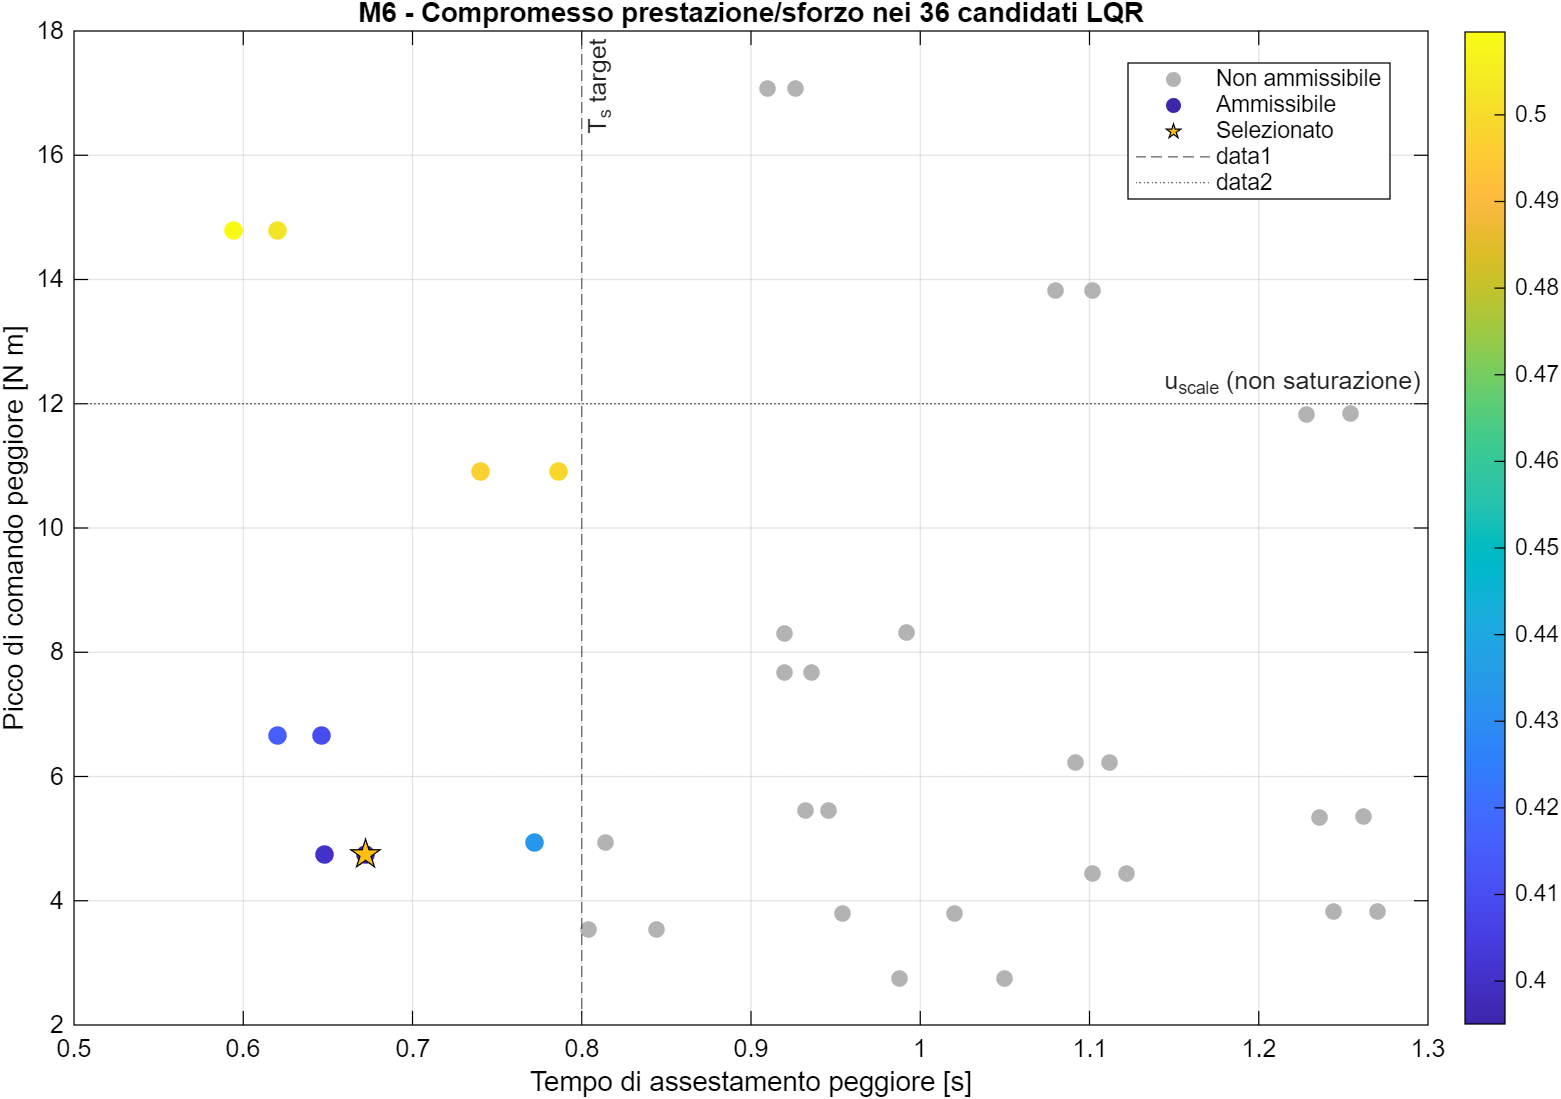
\includegraphics[width=0.78\textwidth]{figures/m6_lqr_candidate_tradeoff.png}
\caption{Ogni punto deriva dai due gradini nominali di un candidato LQR:
ascissa $T_s$ peggiore, ordinata picco di coppia; il colore indica lo score dei
candidati ammissibili e il simbolo evidenzia quello selezionato.
La linea a 12 N m è una scala, non una saturazione.}
\label{fig:m6-lqr-search}
\end{figure}
\begin{figure}[H]\centering
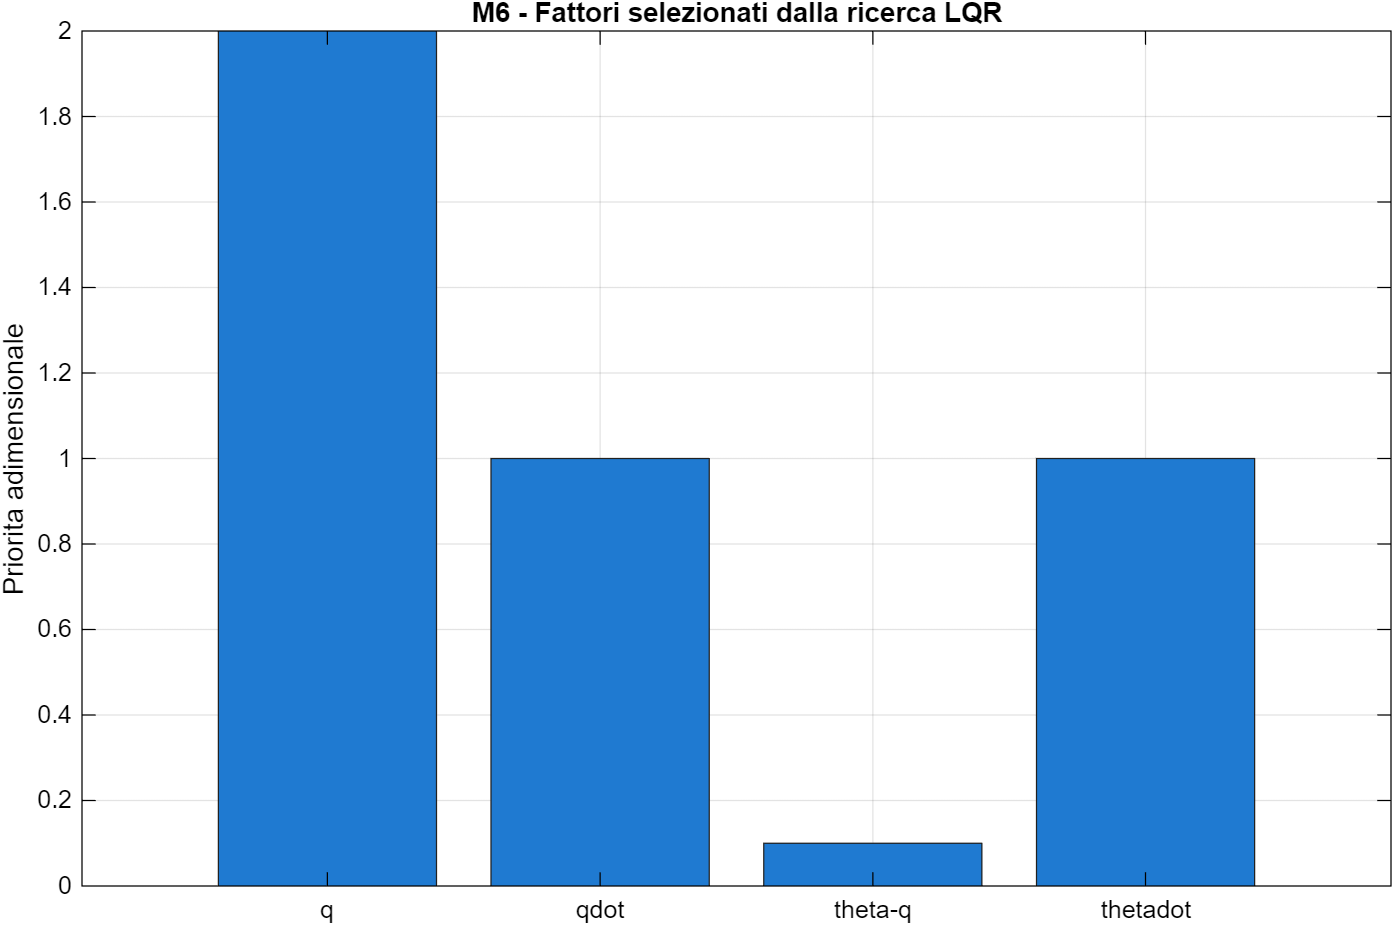
\includegraphics[width=0.70\textwidth]{figures/m6_lqr_selected_weights.png}
\caption{Priorità adimensionali selezionate, da non confondere con le scale fisiche
né con i singoli elementi della matrice non diagonale $Q$.}\label{fig:m6-lqr-weights}
\end{figure}

\subsection{Q e R finali, Riccati, guadagno e stabilità}
MATLAB risolve l'equazione algebrica di Riccati:
\[
A^TP_{\mathrm{LQR}}+P_{\mathrm{LQR}}A
-P_{\mathrm{LQR}}BR^{-1}B^TP_{\mathrm{LQR}}+Q=0,\qquad
K=R^{-1}B^TP_{\mathrm{LQR}}.
\]
$P_{\mathrm{LQR}}$ non è la matrice di Lyapunov introdotta nel Capitolo 10.
Le matrici seguenti provengono dallo script eseguito, arrotondate a cinque cifre
significative; gli artifact conservano la doppia precisione.
% Generato da build_technical_revision_tables, non modificare.
\[Q=\operatorname{blkdiag}(Q_8,0_{6\times6}),\qquad R=\tfrac{1}{9}I_2.\]
{\small
\[
Q_8=\begin{bmatrix}
902.62 & 0 & 0 & 0 & -640 & 0 & 0 & 0 \\
0 & 902.62 & 0 & 0 & 0 & -640 & 0 & 0 \\
0 & 0 & 0.91189 & 0 & 0 & 0 & 0 & 0 \\
0 & 0 & 0 & 0.91189 & 0 & 0 & 0 & 0 \\
-640 & 0 & 0 & 0 & 640 & 0 & 0 & 0 \\
0 & -640 & 0 & 0 & 0 & 640 & 0 & 0 \\
0 & 0 & 0 & 0 & 0 & 0 & 0.91189 & 0 \\
0 & 0 & 0 & 0 & 0 & 0 & 0 & 0.91189 \\
\end{bmatrix}
\]
\[K=[K_a\ K_b],\quad K_a=K(:,1{:}7),\quad K_b=K(:,8{:}14).\]
\[
K_a=\begin{bmatrix}
238.32 & 15.153 & 18.091 & 3.653 & -154.27 & -12.282 & -1.2845 \\
14.6 & 200.59 & 4.4912 & 7.0445 & -5.6235 & -133.66 & -0.61277 \\
\end{bmatrix}
\]
\[
K_b=\begin{bmatrix}
-0.87229 & 11.16 & 21.126 & 39.687 & -0.96424 & -2.3084 & -12.957 \\
1.2023 & -0.96424 & -2.1764 & -10.461 & 13.925 & 27.556 & 75.884 \\
\end{bmatrix}
\]
\[
N_r=\begin{bmatrix}
51.688 & -1.1626 \\
3.2384 & 49.052 \\
\end{bmatrix}
\]
}

La norma del residuo CARE è \RevCareResidual; il polo dominante del regolatore
ha parte reale $-\RevRegulatorDecay$ s$^{-1}$. Tutti i poli di $A-BK$ sono
strettamente nel semipiano sinistro. Il collegamento verificato è dunque
$Q,R\to P_{\mathrm{LQR}}\to K\to A-BK\to$ risposte temporali.
Il prefiltro è $N_r=[-C_q(A-BK)^{-1}B]^{-1}$: garantisce tracking statico
nominale, non reiezione esatta di disturbi costanti.

\section{Filtro di Kalman: ipotesi, covarianze e verifica}
\subsection{Stima dello stato e innovazione}
LQR richiede $x$, mentre sono disponibili soltanto le quattro posizioni.
Il modello usato per la stima è
\[
\dot x=Ax+Bu+G_ww,\qquad y=Cx+v,\qquad G_w=[B_d\ B].
\]
I primi due canali di $w$ sono coppie equivalenti lato link, i successivi due
coppie equivalenti all'ingresso attuativo. I quattro canali di $v$ rappresentano
gli encoder di $q$ e $\theta$. Sono ipotizzati indipendenti, a media nulla,
senza correlazione processo--misura. Lo stimatore realizza
\[
\dot{\hat x}=A\hat x+Bu+L(y-C\hat x).
\]
L'innovazione $y-C\hat x$ confronta la misura con la previsione del modello:
il guadagno $L$ stabilisce quanto questa differenza corregga ciascuno stato.

\subsection{Origine delle sigma e costruzione non ambigua delle covarianze}
Non sono disponibili dati sperimentali sui sensori o sugli errori di processo.
Le scale
$\sigma_d=0.1$ N m, $\sigma_u=0.1$ N m e $\sigma_y=0.05^\circ$
sono ipotesi progettuali D di questo lavoro, \emph{non dati del docente}.
Il loro scopo è assegnare fiducia relativa al modello e alle misure, non
rappresentare una caratterizzazione dell'hardware.
Per contestualizzarle, 0.1 N m equivale al 20\% del disturbo M5 e allo 0.83\%
della scala di comando; 0.05 gradi equivale all'1\% del riferimento.
Questi rapporti descrivono i valori già scelti: non sono una legge fisica che
li determini univocamente. La sensibilità successiva ne rende verificabili
le conseguenze senza un'ottimizzazione delle covarianze.

La varianza è il quadrato della deviazione standard. La costruzione effettiva è
\[
Q_n=\operatorname{diag}(\sigma_d^2,\sigma_d^2,\sigma_u^2,\sigma_u^2)
=0.01\,I_4,\qquad
R_n=(0.05\pi/180)^2I_4=\RevRn\,I_4.
\]
$Q_n$ agisce sui quattro canali di $w$, non direttamente sui 14 stati;
la covarianza equivalente nello stato è $G_wQ_nG_w^T$.
La notazione $0.01 I_4$ evita ogni ambiguità fra $(0.1)^2$ e $0.12$.

Una precisazione è necessaria per il filtro continuo: il rumore bianco ideale
non ha una deviazione standard istantanea finita. In \texttt{lqe}, $Q_n,R_n$
sono intensità, ossia coefficienti della delta di Dirac nelle correlazioni.
Le sigma sopra sono scale equivalenti riferite alla convenzione temporale di
1 s; restituendo le dimensioni temporali, le intensità hanno unità
$(\mathrm{N\,m})^2\,\mathrm{s}$ e $\mathrm{rad}^2\,\mathrm{s}$.
La successiva simulazione \texttt{randn} usa invece campioni con deviazione
standard finita a passo 2 ms. Non viene affermata l'equivalenza di questo
esperimento con il modello bianco continuo né una calibrazione probabilistica.

\subsection{Guadagno, poli e sensibilità a ingresso identico}
Il calcolo eseguito è
$\texttt{L=lqe(A,Gw,C,Qn,Rn)}$. La matrice seguente segue l'ordine degli stati
M3 per le righe e $[q_1,q_2,\theta_1,\theta_2]$ per le colonne:
{\small
\[
L=\begin{bmatrix}
22.709 & -21.794 & 9.0441 & -5.5227 \\
-21.794 & 85.604 & -6.9226 & 23.471 \\
551.47 & -1274.4 & 233.27 & -349.38 \\
-1278.4 & 4200.9 & -381.6 & 1210.6 \\
9.0441 & -6.9226 & 64.38 & -3.4219 \\
-5.5227 & 23.471 & -3.4219 & 79.196 \\
724.13 & -934.1 & 2143.1 & -313.45 \\
-755.87 & 2801.5 & -390.28 & 3432.6 \\
-0.41526 & -2.2541 & -35.115 & -1.7286 \\
24.32 & 14.409 & -92.137 & -0.28863 \\
-30.066 & -12.673 & 207.83 & 4.7948 \\
-1.9579 & 4.8133 & -1.7025 & -30.032 \\
11.54 & -9.1651 & 1.3605 & -101.99 \\
-9.7589 & -0.59062 & 2.617 & 207.42 \\
\end{bmatrix}
\]
}

I poli di $A-LC$ sono stabili; la velocità asintotica minima vale
$\alpha_e=\RevEstimatorDecay$ s$^{-1}$, contro
$\alpha_c=\RevRegulatorDecay$ s$^{-1}$ del regolatore.
Il rapporto è \MKalmanSpeedRatio, non un requisito imposto dal docente.

Nella nuova verifica si varia soltanto il rumore \emph{assunto} dallo stimatore:
$0.5\sigma_y,\sigma_y,2\sigma_y$, cioè $R_n/4,R_n,4R_n$.
$Q_n$ e LQR restano invariati. Si applica a tutti la stessa sequenza encoder,
con $\sigma_y=0.05^\circ$, seed 20260826, 4 s a passo 2 ms, riferimento
$r_1=5^\circ,r_2=0$, stato iniziale nullo e nessun disturbo di coppia.
\begin{table}[H]\centering\small
\begin{tabular}{rrrrr}\toprule
$\sigma_{y,ass}/\sigma_y$ & $\alpha_e/\alpha_c$ & RMS $e_q$ [rad] & RMS $\Delta u$ [N m] & $\|G_{v\to C_{cost}e}\|_2$ \\
\midrule
0.5 & 2.0962 & 0.00029595 & 0.14991 & 1065.8 \\
1 & 1.4985 & 0.00023377 & 0.08195 & 718.29 \\
2 & 1.1833 & 0.00018109 & 0.042779 & 486.49 \\
\bottomrule\end{tabular}
\caption{Sensibilit\`a a parit\`a di rumore applicato: seed 20260826, $\sigma_y=0.05^\circ$, passo 2 ms, 4 s. Varia solo $R_n$ assunto.}\label{tab:kalman-fixed}
\end{table}

Il filtro che assume misure più affidabili è più rapido, ma nella prova
a rumore identico amplifica maggiormente le fluttuazioni di stima e comando.
Aumentare relativamente $R_n$ tende a filtrare di più; aumentare relativamente
$Q_n$ tende a valorizzare l'innovazione. Questa è una tendenza complessiva:
nel caso MIMO non implica monotonia di ogni polo o elemento di $L$.
La norma $\mathcal H_2$ è quella della mappa
$v\to C_{cost}(x-\hat x)$ a ingresso unitario, non un RMS fisico del sensore.

L'esperimento precedente, conservato nelle colonne storiche dell'artifact,
variava anche l'ampiezza del rumore applicato: confrontava scenari diversi.
Le nuove colonne \texttt{RmsEstimationErrorFixedNoise} e
\texttt{RmsControlFixedNoise} isolano invece l'effetto della sola covarianza assunta.
\begin{figure}[H]\centering
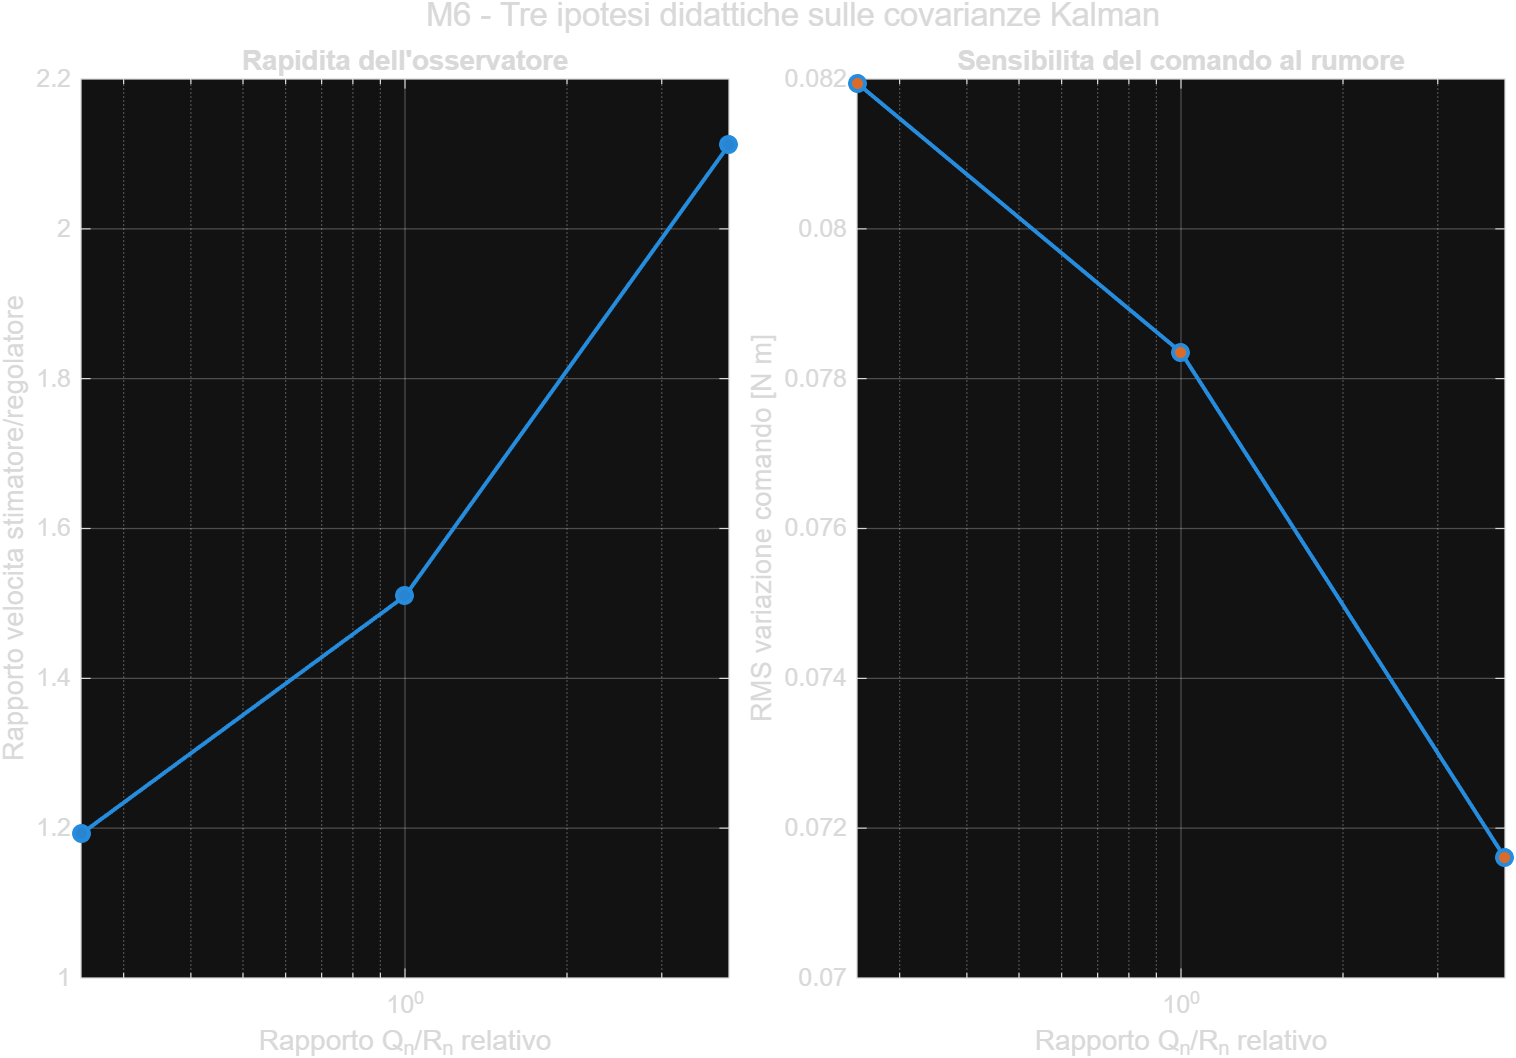
\includegraphics[width=0.84\textwidth]{figures/m6_kalman_sensitivity.png}
\caption{A sinistra, rapidità relativa dello stimatore; a destra, RMS della
variazione di coppia a rumore applicato identico. L'ascissa è il rapporto
$Q_n/R_n$ relativo al progetto nominale, non un rapporto adimensionale
fra grandezze fisiche eterogenee.}\label{fig:m6-kalman-sensitivity}
\end{figure}

\subsection{LQG e principio di separazione}
Per $z=[x^T,\hat x^T]^T$ la matrice completa è
\[
A_{cl}=\begin{bmatrix}A&-BK\\LC&A-BK-LC\end{bmatrix}.
\]
Con $e=x-\hat x$ si ottiene la forma triangolare
\[
\begin{bmatrix}\dot x\\\dot e\end{bmatrix}
=\begin{bmatrix}A-BK&BK\\0&A-LC\end{bmatrix}
\begin{bmatrix}x\\e\end{bmatrix}
\]
in assenza di ingressi esogeni. L'unione degli spettri di regolatore e stimatore
coincide quindi con quello della chiusura completa. La trasformazione viene
verificata numericamente nello script; il residuo è \RevSeparation.
Questo risultato riguarda stabilità nominale lineare, non robustezza rispetto
a M4 o stabilità non lineare globale.
\begin{table}[H]\centering\small
\begin{tabular}{rrrr}\toprule
$\Re\lambda(A-BK)$ & $\Im\lambda(A-BK)$ & $\Re\lambda(A-LC)$ & $\Im\lambda(A-LC)$ \\
\midrule
-6.17169 & 3.60433 & -9.31874 & 11.7171 \\
-6.17169 & -3.60433 & -9.31874 & -11.7171 \\
-11.8699 & 0 & -16.1307 & 78.1825 \\
-23.4741 & 86.4634 & -16.1307 & -78.1825 \\
-23.4741 & -86.4634 & -22.0159 & 84.7841 \\
-27.2576 & 43.8044 & -22.0159 & -84.7841 \\
-27.2576 & -43.8044 & -44.873 & 51.743 \\
-28.0575 & 84.428 & -44.873 & -51.743 \\
-28.0575 & -84.428 & -47.6737 & 29.4495 \\
-31.1221 & 0 & -47.6737 & -29.4495 \\
-52.8324 & 0 & -51.9324 & 32.5343 \\
-66.9325 & 0 & -51.9324 & -32.5343 \\
-133.333 & 0 & -133.333 & 0 \\
-133.333 & 0 & -133.333 & 0 \\
\bottomrule\end{tabular}
\caption{Poli in s$^{-1}$. Le due coppie di colonne elencano spettri distinti; le righe non associano un modo del regolatore a uno dello stimatore.}
\end{table}


\section{Risultati M6: lettura delle figure}
\subsection{Tracking del riferimento}
La Figura~\ref{fig:m6-tracking} usa tempo in secondi e deviazioni articolari
in gradi. Nel pannello superiore si applica $r_1=5^\circ,r_2=0$;
in quello inferiore $r_1=0,r_2=5^\circ$. Stato fisico e osservatore partono
da zero; coppie di disturbo e rumore sono nulli.
Le curve continue sono $q_1,q_2$, la tratteggiata il riferimento non nullo.
Si osservano rapidità del giunto comandato, picco del giunto non comandato e
raggiungimento del valore finale. Il peggiore $T_s$ è \MControllerWorstTs\ s:
M6 soddisfa i target nominali, pur senza disaccoppiamento perfetto.
\begin{figure}[H]\centering
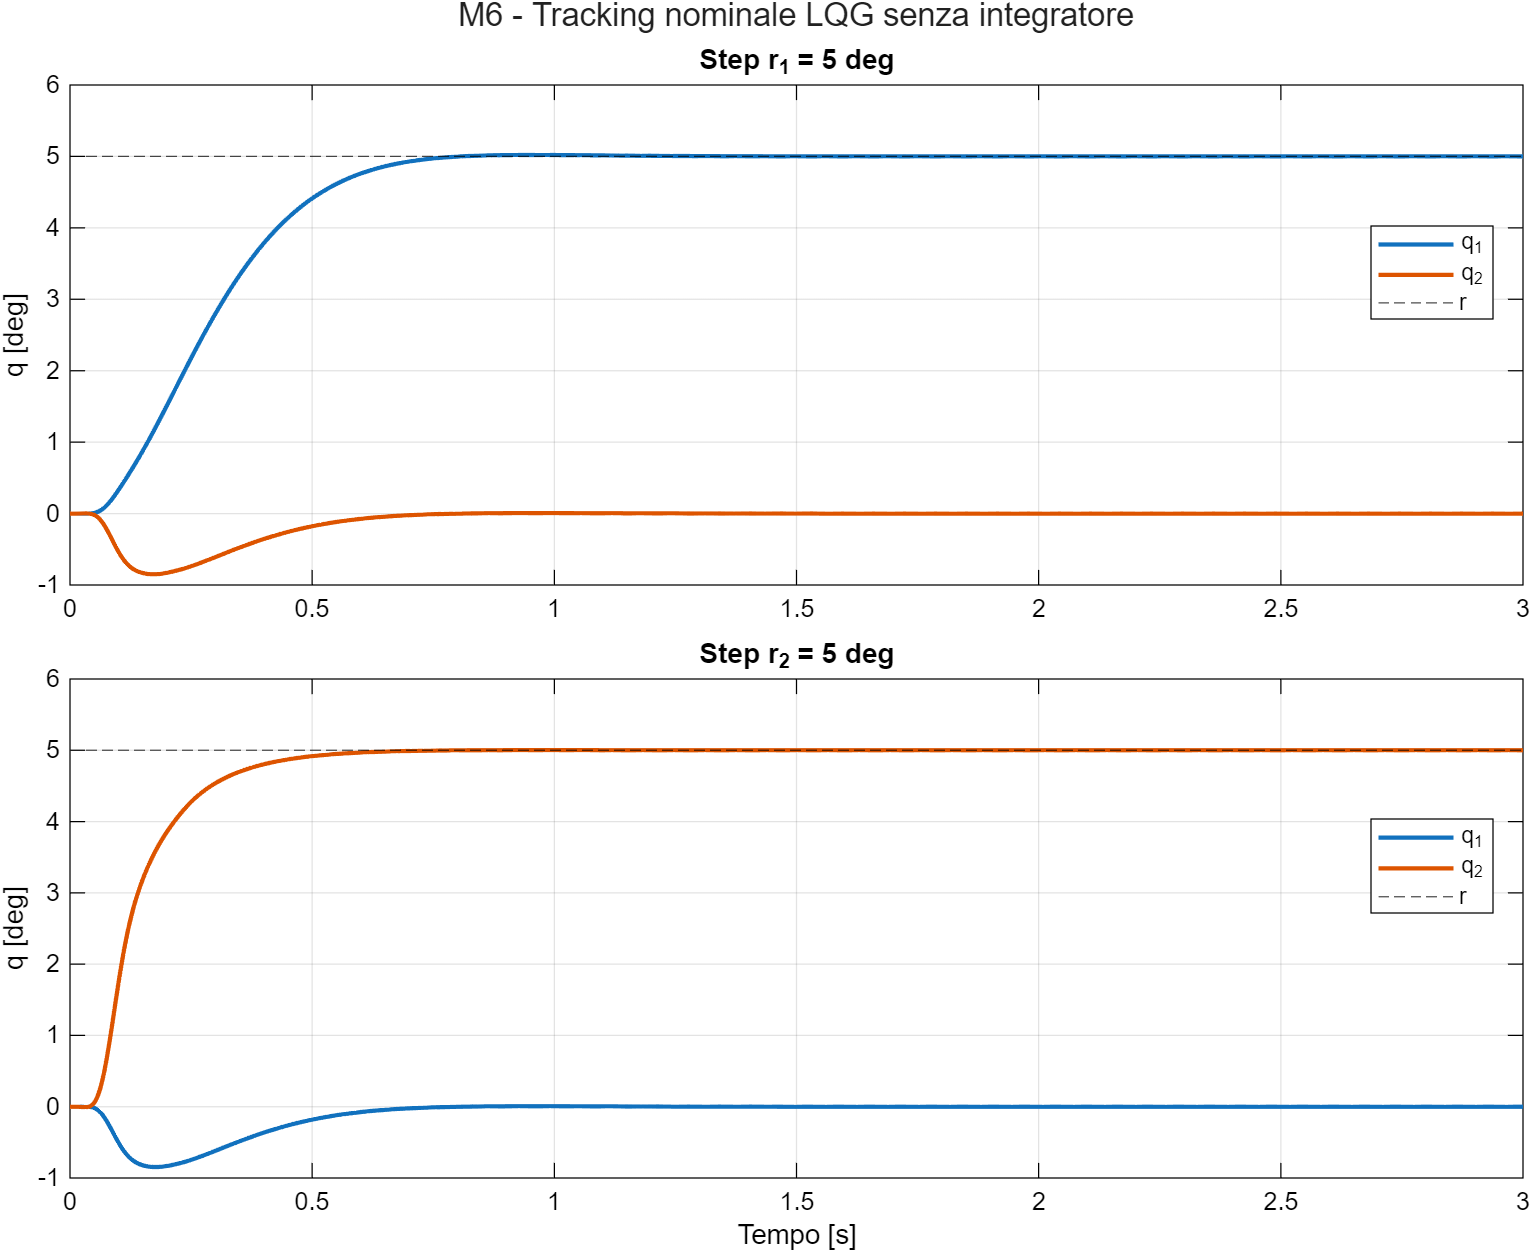
\includegraphics[width=0.82\textwidth]{figures/m6_lqg_reference_tracking.png}
\caption{Due prove di tracking nominale LQG a gradino di 5 gradi, senza disturbi
o rumore e da condizioni iniziali nulle.}\label{fig:m6-tracking}
\end{figure}

\subsection{Disturbo costante e limite del prefiltro}
Nella Figura~\ref{fig:m6-disturbo} il riferimento è nullo e si applica da $t=0$
una coppia costante di 0.5 N m al primo link (sopra) o al secondo (sotto).
Il rumore è nullo e gli stati iniziali sono nulli. Le curve riportano le due
deviazioni di posizione in gradi nel tempo. L'offset non nullo non è un errore
del grafico: il prefiltro corregge il guadagno statico sul riferimento,
non introduce l'azione integrale necessaria alla reiezione esatta.
\begin{figure}[H]\centering
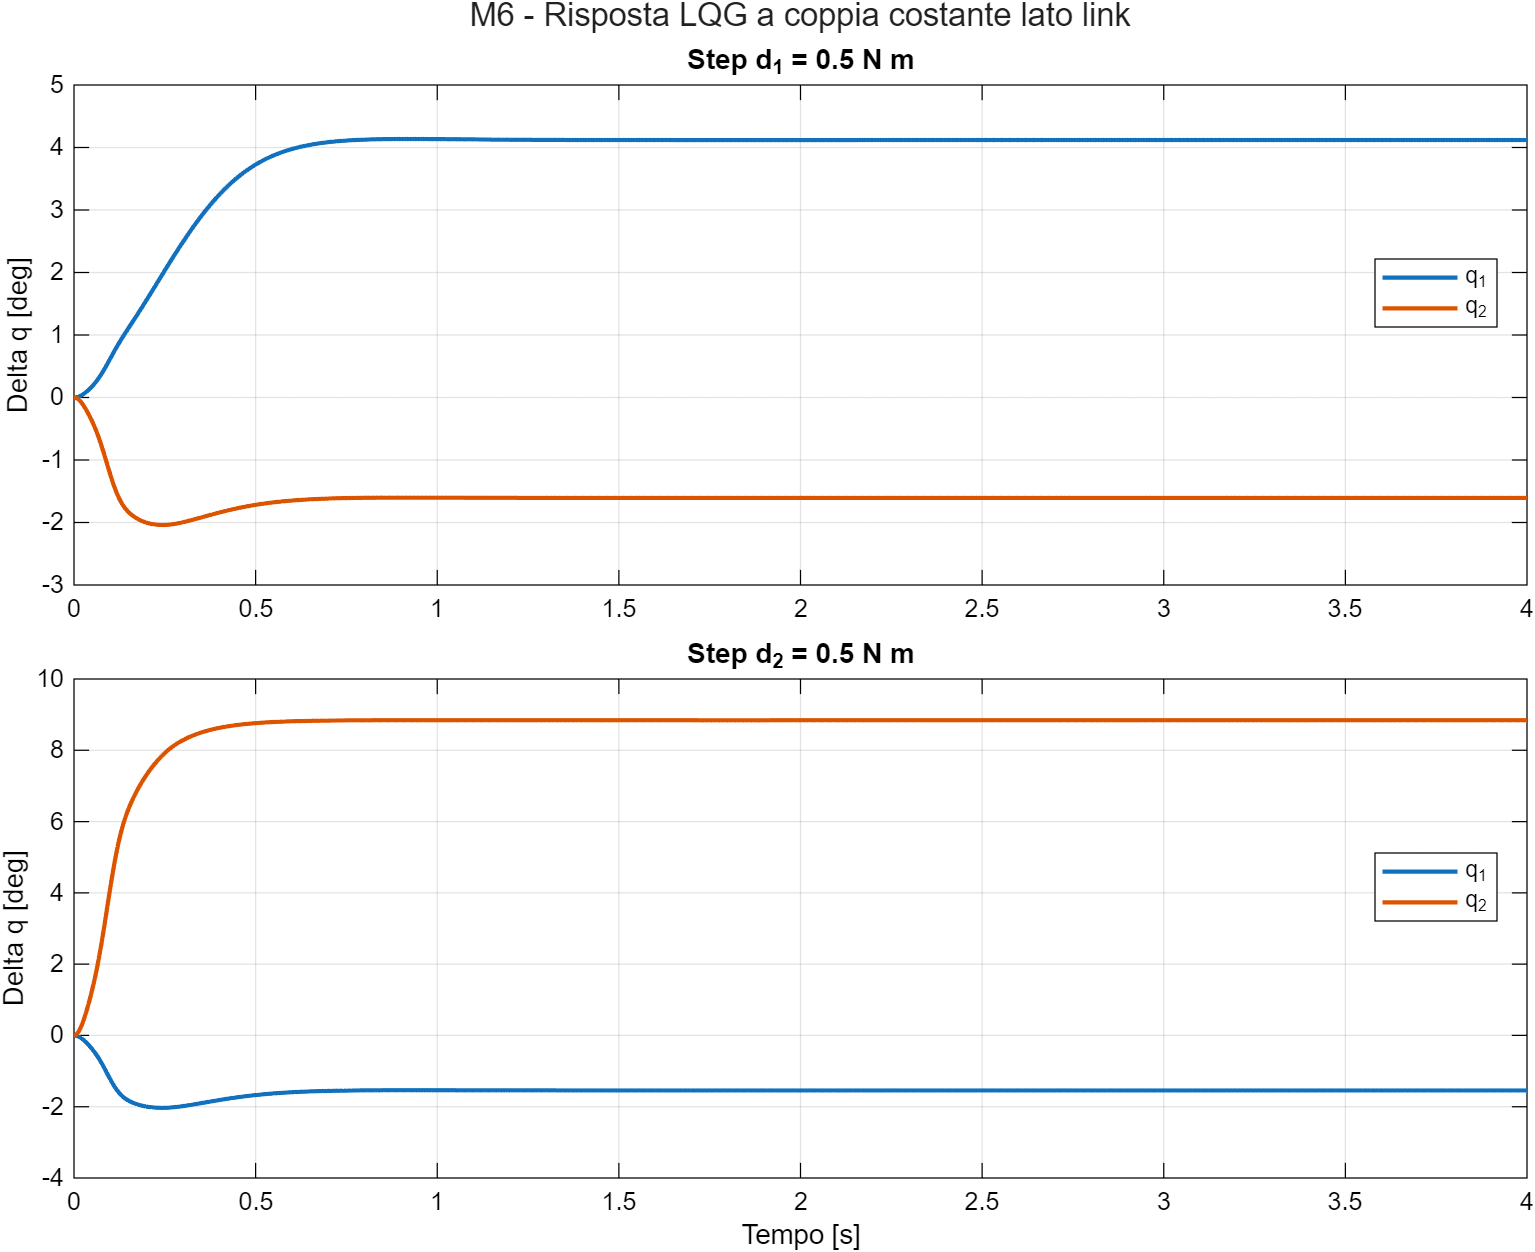
\includegraphics[width=0.82\textwidth]{figures/m6_lqg_disturbance_response.png}
\caption{Risposta ai due gradini di coppia lato link: il recupero resta stabile,
ma permane un offset coerente con l'assenza di integratori.}\label{fig:m6-disturbo}
\end{figure}

\subsection{Errore di stima e rumore sul comando}
La Figura~\ref{fig:m6-stima} usa lo scenario seeded di 4 s:
$r_1=5^\circ,r_2=0$, nessuna coppia disturbante, stati iniziali nulli
e rumore sui quattro encoder di deviazione standard 0.05 gradi.
Sopra si leggono $q_i-\hat q_i$ in gradi; sotto la differenza fra le coppie
della prova rumorosa e quelle della stessa prova senza rumore, in N m.
Non è quindi il comando totale. Le oscillazioni residue quantificano il
compromesso fra inseguimento delle misure e filtraggio.
\begin{figure}[H]\centering
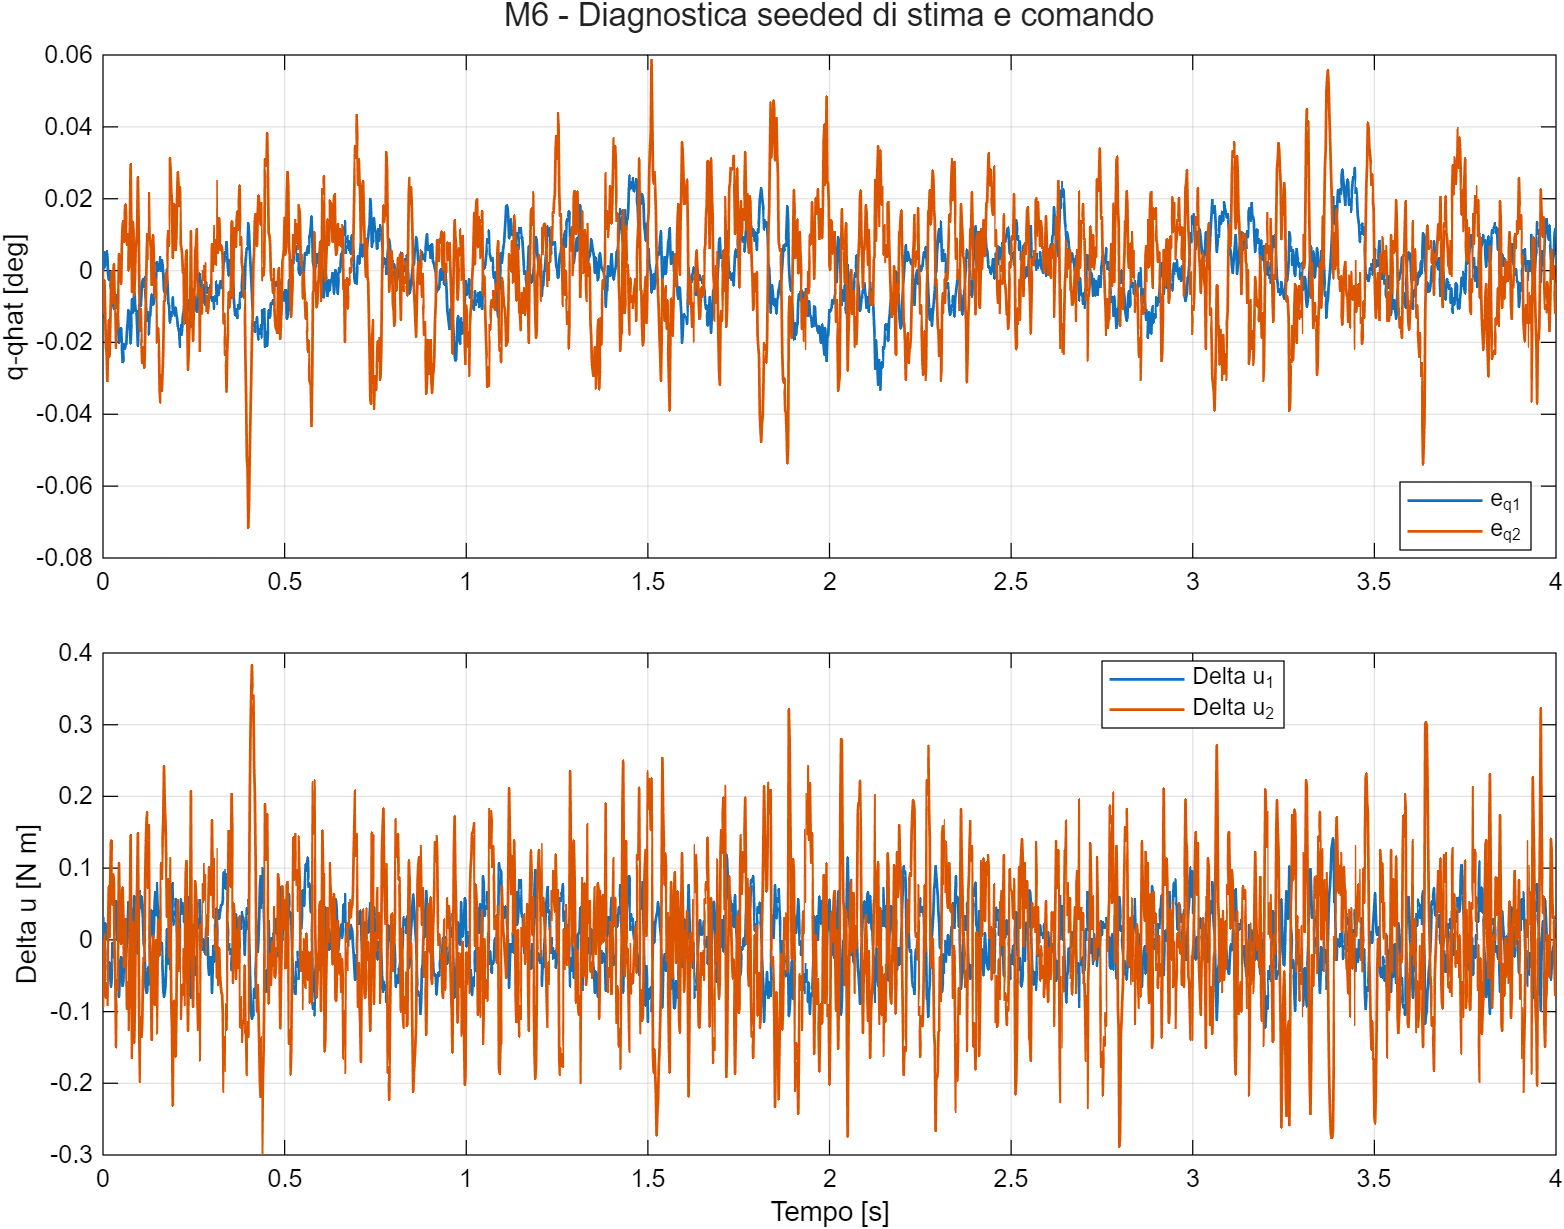
\includegraphics[width=0.82\textwidth]{figures/m6_lqg_estimation.png}
\caption{Errore sui due stati di posizione stimati e incremento di coppia
imputabile alla sequenza di rumore encoder, a riferimento identico.}\label{fig:m6-stima}
\end{figure}

\subsection{Poli e portata delle conclusioni}
La Figura~\ref{fig:m6-poli} non è una simulazione temporale: ascisse e ordinate
sono le parti reale e immaginaria dei poli in s$^{-1}$.
Non richiede condizioni iniziali, riferimenti o disturbi.
I simboli separano regolatore, stimatore e chiusura aumentata; la sovrapposizione
verifica il principio di separazione e la posizione a sinistra dell'asse
immaginario verifica la stabilità nominale.
\begin{figure}[H]\centering
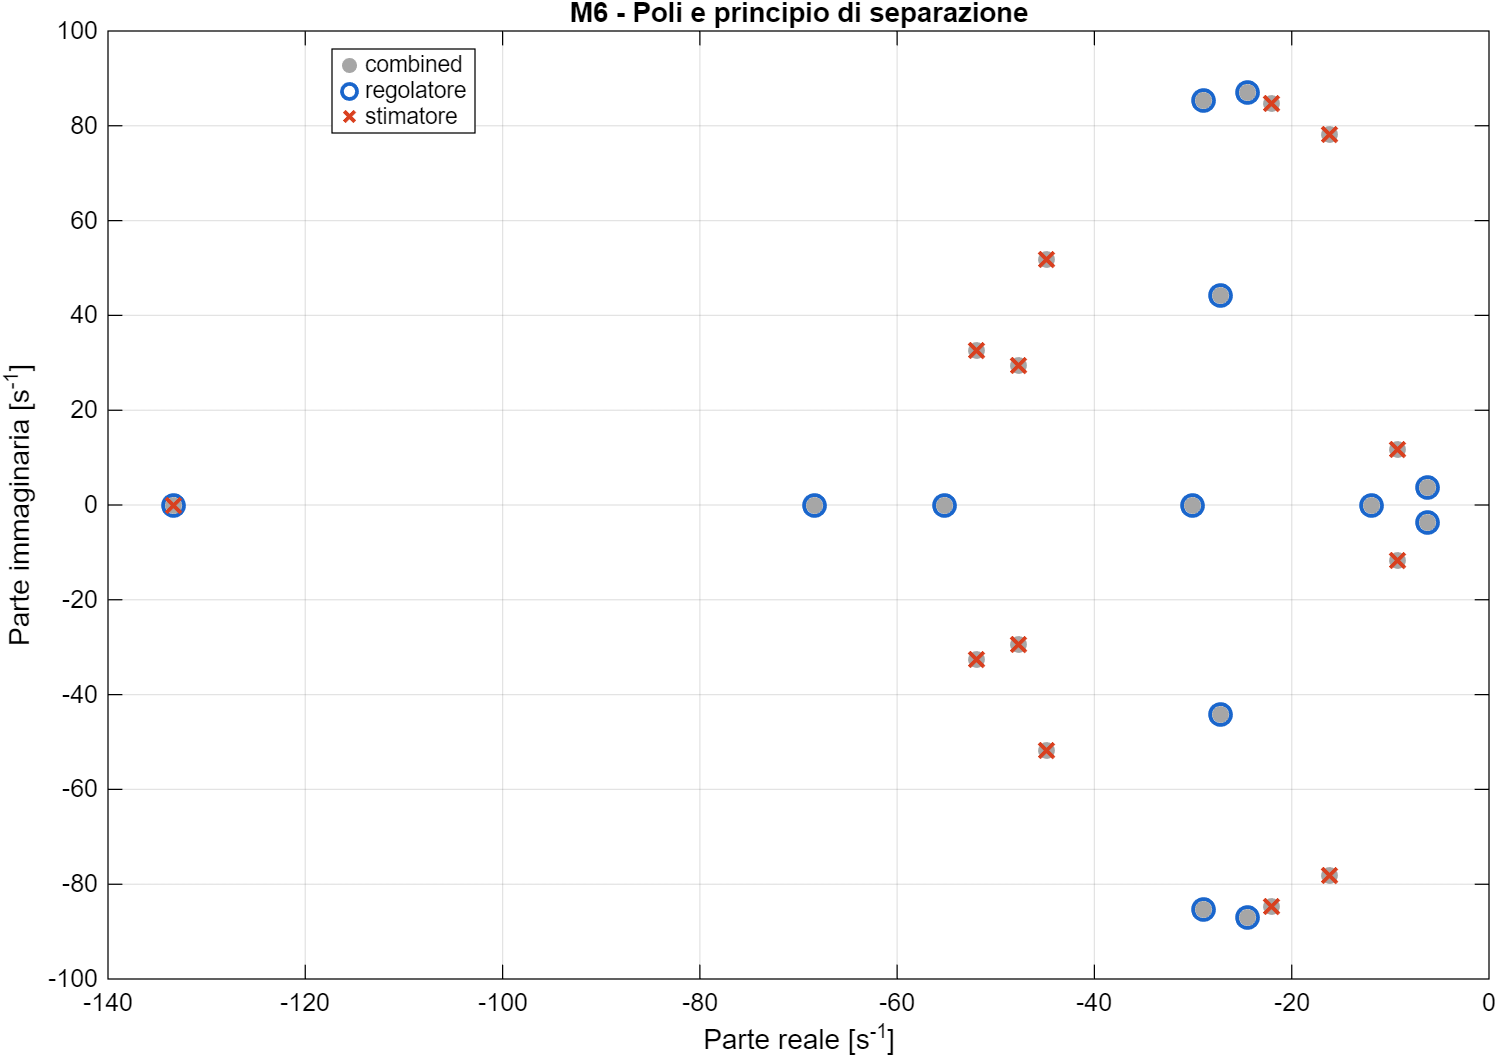
\includegraphics[width=0.80\textwidth]{figures/m6_lqg_poles.png}
\caption{Spettri del regolatore, dello stimatore e della chiusura LQG completa,
senza cancellazioni di stati.}\label{fig:m6-poli}
\end{figure}
Il comando full-state usato nella selezione ha picco peggiore
\MLqrPeakControl\ N m e RMS \MLqrRmsControl\ N m.
La verifica non lineare e il limite interno di Lyapunov, che includono
l'osservatore, sono sviluppati nel Capitolo 10; non sono dedotti dai soli poli.

\section{Implementazione Simulink didattica}
Il modello \texttt{SEA\_LQG\_nonlinear.slx} mostra al livello superiore sei blocchi funzionali: riferimento, controllore LQG, dinamica degli attuatori, pianta SEA non lineare, interfaccia di misura e monitoraggio. Dentro il controllore sono separati il prefiltro $N_r$, il feedback $-K\hat x$, la somma che genera il comando incrementale e l'osservatore di Kalman. Quest'ultimo realizza
\[
\dot{\hat x}=(A-LC)\hat x+B\,\delta u+L\,\delta y,
\qquad \delta u=-K\hat x+N_rr.
\]
L'interfaccia di misura estrae soltanto $q$ e $\theta$, sottrae l'equilibrio e aggiunge il rumore encoder; le velocità non vengono misurate. La coppia assoluta inviata agli attuatori è $u_{abs}=\bar\tau+\delta u$. Tutti i guadagni sono incorporati dall'artifact M6 validato e le condizioni iniziali vengono passate con \texttt{SimulationInput}; il modello non dipende dal base workspace. Non sono presenti saturazioni.

\section{Azione integrale e verifica LQI M7}
\label{sec:lqi}
\subsection{Dall'offset alla memoria dell'errore}
Le simulazioni precedenti mostrano il limite del solo prefiltro. La legge
$\delta u=-K\hat x+N_rr$ corregge il guadagno statico nominale da riferimento
a posizione, ma $N_r$ moltiplica soltanto $r$: non riceve l'errore prodotto
da una coppia disturbante. A riferimento nullo il suo contributo è nullo,
anche se $q$ converge a una posizione diversa dall'equilibrio.

Per le due posizioni articolari incrementali definiamo
\[
e(t)=r(t)-q(t)=r(t)-C_qx(t),\qquad
\xi(t)=\int_0^t e(\tau)\,d\tau,\qquad \dot\xi=r-C_qx,\quad \xi(0)=0.
\]
Ogni componente di $\xi$ è misurata in rad\,s. Un errore positivo fa crescere
la corrispondente componente; uno negativo la fa diminuire. Se l'errore
persiste, il suo integrale continua ad accumularsi: il regolatore dispone
così di una memoria del disallineamento. Un offset costante non può essere
compatibile con un equilibrio finito dell'intero sistema, perché in un
equilibrio deve essere anche $\dot\xi=0$.

Questa è l'applicazione del principio del modello interno ai segnali
costanti: si inseriscono due modi integrali, uno per uscita regolata.
Se la chiusura aumentata è stabile, ammette l'equilibrio richiesto e il
comando non è limitato da saturazioni, il regime costante ha $q=r$.
La correzione $-K_i\xi$ può restare non nulla anche dopo che $e$ si è
annullato: è proprio il contributo permanente necessario a bilanciare
il disturbo. Non si afferma invece che l'errore sia nullo durante il
transitorio o che il risultato valga automaticamente per il sistema incerto.

\subsection{Il sistema aumentato effettivo: 14 più 2 stati}
La pianta è ancora M3, con $A\in\mathbb R^{14\times14}$,
$B\in\mathbb R^{14\times2}$ e $C_q\in\mathbb R^{2\times14}$.
Lo stato $x$ comprende gli otto stati meccanici e i sei stati attuativi
già descritti; non vengono eliminati gli attuatori. Ponendo
$x_a=[x^T,\xi^T]^T\in\mathbb R^{16}$ si ottiene
\[
\begin{bmatrix}\dot x\\\dot\xi\end{bmatrix}
=
\underbrace{\begin{bmatrix}A&0_{14\times2}\\-C_q&0_{2\times2}\end{bmatrix}}_{A_a}
\begin{bmatrix}x\\\xi\end{bmatrix}
+\underbrace{\begin{bmatrix}B\\0_{2\times2}\end{bmatrix}}_{B_a}u
+\underbrace{\begin{bmatrix}0_{14\times2}\\I_2\end{bmatrix}}_{B_r}r.
\]
Il disturbo lato link aggiunge $B_{d,a}d$, con
$B_{d,a}=[B_d^T,0_{2\times2}]^T$. Le dimensioni di $A_a,B_a,B_r$
sono rispettivamente $16\times16$, $16\times2$, $16\times2$.

L'aggiunta degli integratori non è innocua: se un modo non stabile non
è controllabile, Riccati non può fornire un regolatore stabilizzante.
Il costruttore \texttt{build\_lqi\_augmented\_cost.m} verifica
\[
\operatorname{rank}\,[\lambda I_{16}-A_a\;\;B_a]=16
\quad\text{per i poli con }\Re\lambda\geq-10^{-8}.
\]
Il test PBH all'origine restituisce 16, come il rango della matrice
di Rosenbrock
\[
\operatorname{rank}\begin{bmatrix}A&B\\C_q&0\end{bmatrix}=16.
\]
Non vi è quindi un'ostruzione dovuta a zeri invarianti nell'origine.
Questi controlli sono preferibili a interpretare ingenuamente il solo
rango numerico di \texttt{ctrb}, sensibile allo scaling e alle potenze di $A_a$.

\subsection{Costo, scala integrale e significato di \texorpdfstring{$w_i$}{wi}}
Il problema risolto è
\[
J_{\rm LQI}=\int_0^\infty
\left(x^TQx+\xi^TQ_i\xi+u^TRu\right)dt
=\int_0^\infty\left(x_a^TQ_ax_a+u^TRu\right)dt,
\qquad Q_a=\operatorname{blkdiag}(Q,Q_i).
\]
Il blocco $Q$ è esattamente quello M6, inclusi i termini non diagonali.
Il codice adotta
\[
s_\xi=q_sT_{s,\mathrm{target}}
=(5\pi/180)\,0.8\ {\rm rad\,s},\qquad
Q_i=\frac{w_i}{s_\xi^2}I_2,\qquad
R=\frac{\rho_U}{u_{\mathrm{scale}}^2}I_2.
\]
La scala $s_\xi$ è derivata dai target progettuali M5: rappresenta
l'accumulo di un errore pari a $q_s$ per un tempo pari al settling richiesto.
Non è una misura sperimentale né un limite fisico dell'integratore.
Invece $w_i$ è una priorità adimensionale di tuning: pesa
$\|\xi/s_\xi\|^2$ nel costo, senza cambiare la scala o il requisito M5.

Con $w_i$ piccolo l'accumulo costa relativamente poco; con $w_i$ grande
il problema LQR tende a contrastarlo maggiormente. Ci si attende in genere
una correzione integrale più rapida, ma anche possibili aumenti di
sovraelongazione e comando. Non è una monotonicità garantita per qualsiasi
sistema MIMO. Non esiste pertanto un unico $w_i$ teoricamente corretto:
dipende dal compromesso che si intende studiare.

I tre casi originali sono $(w_i,\rho_U)=(0.1,16),(1,8),(4,4)$,
denominati debole, intermedio e forte. Non sono tre prove a parità di $R$:
all'aumento di $w_i$ si accompagna una riduzione della penalizzazione
del comando. Non si può attribuire l'intera variazione delle prestazioni
al solo integratore. Una verifica diagnostica aggiuntiva mantiene invece
$\rho_U=16$ e lo stesso $Q$: per $w_i=0.1,1,4$ si ottengono
$\|K_i\|_2=13.589,\ 42.972,\ 85.944$ e parti reali dominanti
$-0.2610,\ -0.8307,\ -1.6975$ s$^{-1}$. In queste tre prove l'azione
integrale cresce e il modo lento accelera; i punti originali M7 non
vengono sostituiti né viene effettuata una nuova selezione del controllore.

\subsection{Da Riccati a \texorpdfstring{$K_x$ e $K_i$}{Kx e Ki}: convenzione di segno}
Fissati $Q,Q_i,R$, MATLAB risolve
\[
A_a^TP_a+P_aA_a-P_aB_aR^{-1}B_a^TP_a+Q_a=0,
\qquad
K_a=R^{-1}B_a^TP_a=[K_x\;\;K_i].
\]
La chiamata è \texttt{[Kaug,Pa,poli]=lqr(Aaug,Baug,Qaug,R)}:
$K_a$ ha dimensione $2\times16$, $K_x$ è $2\times14$ e $K_i$ è
$2\times2$. $K_i$ non è scelto a mano. La catena è
\[
Q,Q_i,R\ \longrightarrow\ Q_a\ \longrightarrow\ P_a\
\longrightarrow\ K_a\ \longrightarrow\ (K_x,K_i).
\]
Con $\dot\xi=r-q$ la legge effettiva M7 è
\[
u=-K_xx-K_i\xi+N_{ff}r,\qquad
N_{ff}=[-C_q(A-BK_x)^{-1}B]^{-1}.
\]
Il prefiltro è ricalcolato da $K_x$, non copiato da M6.
Nel punto intermedio le diagonali di $K_i$ sono negative: il meno
davanti a $K_i\xi$ non va cancellato o reinterpretato. La sua correttezza
è verificata dalla matrice chiusa
\[
A_{\rm LQI}=
\begin{bmatrix}A-BK_x&-BK_i\\-C_q&0\end{bmatrix}
\]
e dall'annullamento della mappa statica $d\mapsto q$.
Per il solo confronto illustrativo si usa il punto intermedio,
$w_i=1,\rho_U=8$, senza promuoverlo a soluzione finale.
Le matrici seguenti e i residui sono esportati dallo script eseguito.
% Generated by plot_lqi_hinf_revision.m.
\[
Q_i=205.18I_2,\qquad R=0.055556I_2,\qquad s_\xi=0.069813\ {\rm rad\,s}.
\]
\[
K_x=[K_{x,a}\ K_{x,b}],\quad K_{x,a}=K_x(:,1{:}7),\quad K_{x,b}=K_x(:,8{:}14).
\]
\[K_{x,a}=\begin{bmatrix}
381.75 & 24.782 & 25.889 & 5.3979 & -248.18 & -18.735 & -1.2107 \\
22.296 & 307.95 & 6.735 & 9.553 & -6.014 & -205.35 & -0.88562 \\
\end{bmatrix}.\]
\[K_{x,b}=\begin{bmatrix}
-1.2396 & 13.998 & 27.737 & 61.323 & -1.0238 & -2.6308 & -16.996 \\
2.3461 & -1.0238 & -2.4981 & -13.938 & 16.824 & 34.815 & 108.21 \\
\end{bmatrix}.\]
\[K_i=\begin{bmatrix}
-60.707 & 2.7917 \\
-2.7917 & -60.707 \\
\end{bmatrix}.\]
\[N_{ff}=\begin{bmatrix}
89.441 & 0.45133 \\
8.1751 & 78.52 \\
\end{bmatrix}.\]
Il residuo relativo dell'ARE è $\num{1.2858e-13}$; $\|K_a-R^{-1}B_a^TP_a\|_F=\num{1.8532e-11}$.
\begin{table}[htbp]\centering\small
\begin{tabular}{rrrrrr}\toprule
$w_i$ & $\rho_U$ & $\|K_i\|_2$ & $T_s$ [s] & OS [\%] & picco $u$ [N m] \\\midrule
0.1 & 16 & 13.589 & \(\infty\) & 7.1007 & 4.8589 \\
1 & 8 & 60.771 & \(\infty\) & 16.585 & 7.8052 \\
4 & 4 & 171.89 & 2.168 & 25.047 & 12.921 \\
\bottomrule\end{tabular}
\caption{Tre punti M7 originali, tracking a 5 gradi su 3 s. $\infty$ significa mancato assestamento entro l'orizzonte, non instabilità.}
\label{tab:lqi-tre-punti}\end{table}
\begin{table}[htbp]\centering\small
\begin{tabular}{llrrrr}\toprule
Controllo & Disturbo & $q_1(\infty)$ & $q_2(\infty)$ & picco $u$ & RMS $u$ \\\midrule
LQG & $d_1$ & 4.1497 & -1.6254 & 1.2932 & 0.7874 \\
LQG & $d_2$ & -1.5621 & 8.9306 & 1.1591 & 0.57365 \\
LQI & $d_1$ & 0 & 0 & 0.87156 & 0.39352 \\
LQI & $d_2$ & 0 & 0 & 1.1324 & 0.37559 \\
\bottomrule\end{tabular}
\caption{Disturbi da 0.5 N m, posizioni asintotiche in gradi e coppie in N m. RMS calcolato su entrambi i comandi negli stessi 8 s.}
\label{tab:lqi-disturbo-numeri}\end{table}


\subsection{Confronto corretto: LQG stimato e LQI a stato vero}
Il confronto non riguarda due architetture con gli stessi sensori.
M6 usa $\hat x$ stimato da $q,\theta$; la verifica M7 usa $x$ vero.
Il sistema chiuso LQG ha 28 stati, mentre il servo LQI ideale ne ha 16.
L'integratore è un'estensione del problema di regolazione, non la
presenza implicita di un filtro Kalman. Un'implementazione sullo stato
stimato richiederebbe esplicitamente $u=-K_x\hat x-K_i\xi+N_{ff}r$
e una nuova verifica della chiusura completa, non effettuata qui.

\begin{table}[H]\centering\small
\begin{tabular}{p{2.7cm}p{5.5cm}p{5.5cm}}\toprule
Aspetto & LQG M6 & LQI M7 illustrativo \\\midrule
Feedback e stato & $-K\hat x+N_rr$; stima Kalman & $-K_xx-K_i\xi+N_{ff}r$; stato vero \\
Memoria dell'errore & Nessun integratore di $r-q$ & Due stati $\xi$ in rad\,s \\
Tracking nominale & Guadagno statico unitario con prefiltro & Guadagno statico unitario nella chiusura stabile \\
Disturbo costante & Offset generalmente non nullo & Offset asintotico nullo nelle prove nominali \\
Complessità & 14 stati di osservatore, 28 chiusi & 2 integratori, 16 chiusi; stato vero richiesto \\
Overshoot e tuning & M6 soddisfa i target nominali & Dipendono da $Q_i,R$; nessun caso M7 rispetta tutti i target \\
Sforzo di controllo & Da valutare per lo scenario & Non cresce necessariamente in ogni prova; confrontare le metriche \\
Saturazioni & Assenti nel modello & Assenti; accumulo e windup possibili in un attuatore reale saturato \\
Vantaggio & Prestazione nominale con misure disponibili & Reiezione nominale dei disturbi costanti \\
Limite & Non elimina l'offset da coppia costante & Settling/overshoot non conformi; servirebbero stima e anti-windup in una realizzazione con saturazioni \\\bottomrule
\end{tabular}
\caption[Confronto delle architetture LQG e LQI]{Differenze fra le architetture effettivamente simulate, non proprietà universali delle sigle LQG e LQI.}
\label{tab:lqg-lqi-logica}
\end{table}

La Figura~\ref{fig:lqi-disturbo} applica due prove separate sul medesimo
modello nominale: $r=0$, condizioni iniziali nulle, nessun rumore,
disturbo a partire da $t=0$ e orizzonte comune di 8 s.
Le colonne distinguono $d=[0.5,0]^T$ e $d=[0,0.5]^T$ N m;
le righe mostrano $q_1$ e $q_2$ in gradi. Ogni asse sovrappone LQG e LQI.
L'offset LQG non è un transitorio incompleto: coincide con il guadagno DC.
LQI converge invece verso zero; a 8 s il massimo residuo osservato
è circa $8.73\cdot10^{-5}$ rad, distinto dallo zero asintotico calcolato.
La Figura~\ref{fig:lqi-comando} usa gli stessi esperimenti e mostra
le coppie incrementali. In queste prove LQI non richiede un picco maggiore
di M6: elimina l'offset con un contributo statico che bilancia la coppia
disturbante. Questo non contraddice i maggiori picchi osservati nel
tracking, che è uno scenario diverso.
\begin{figure}[!htbp]\centering
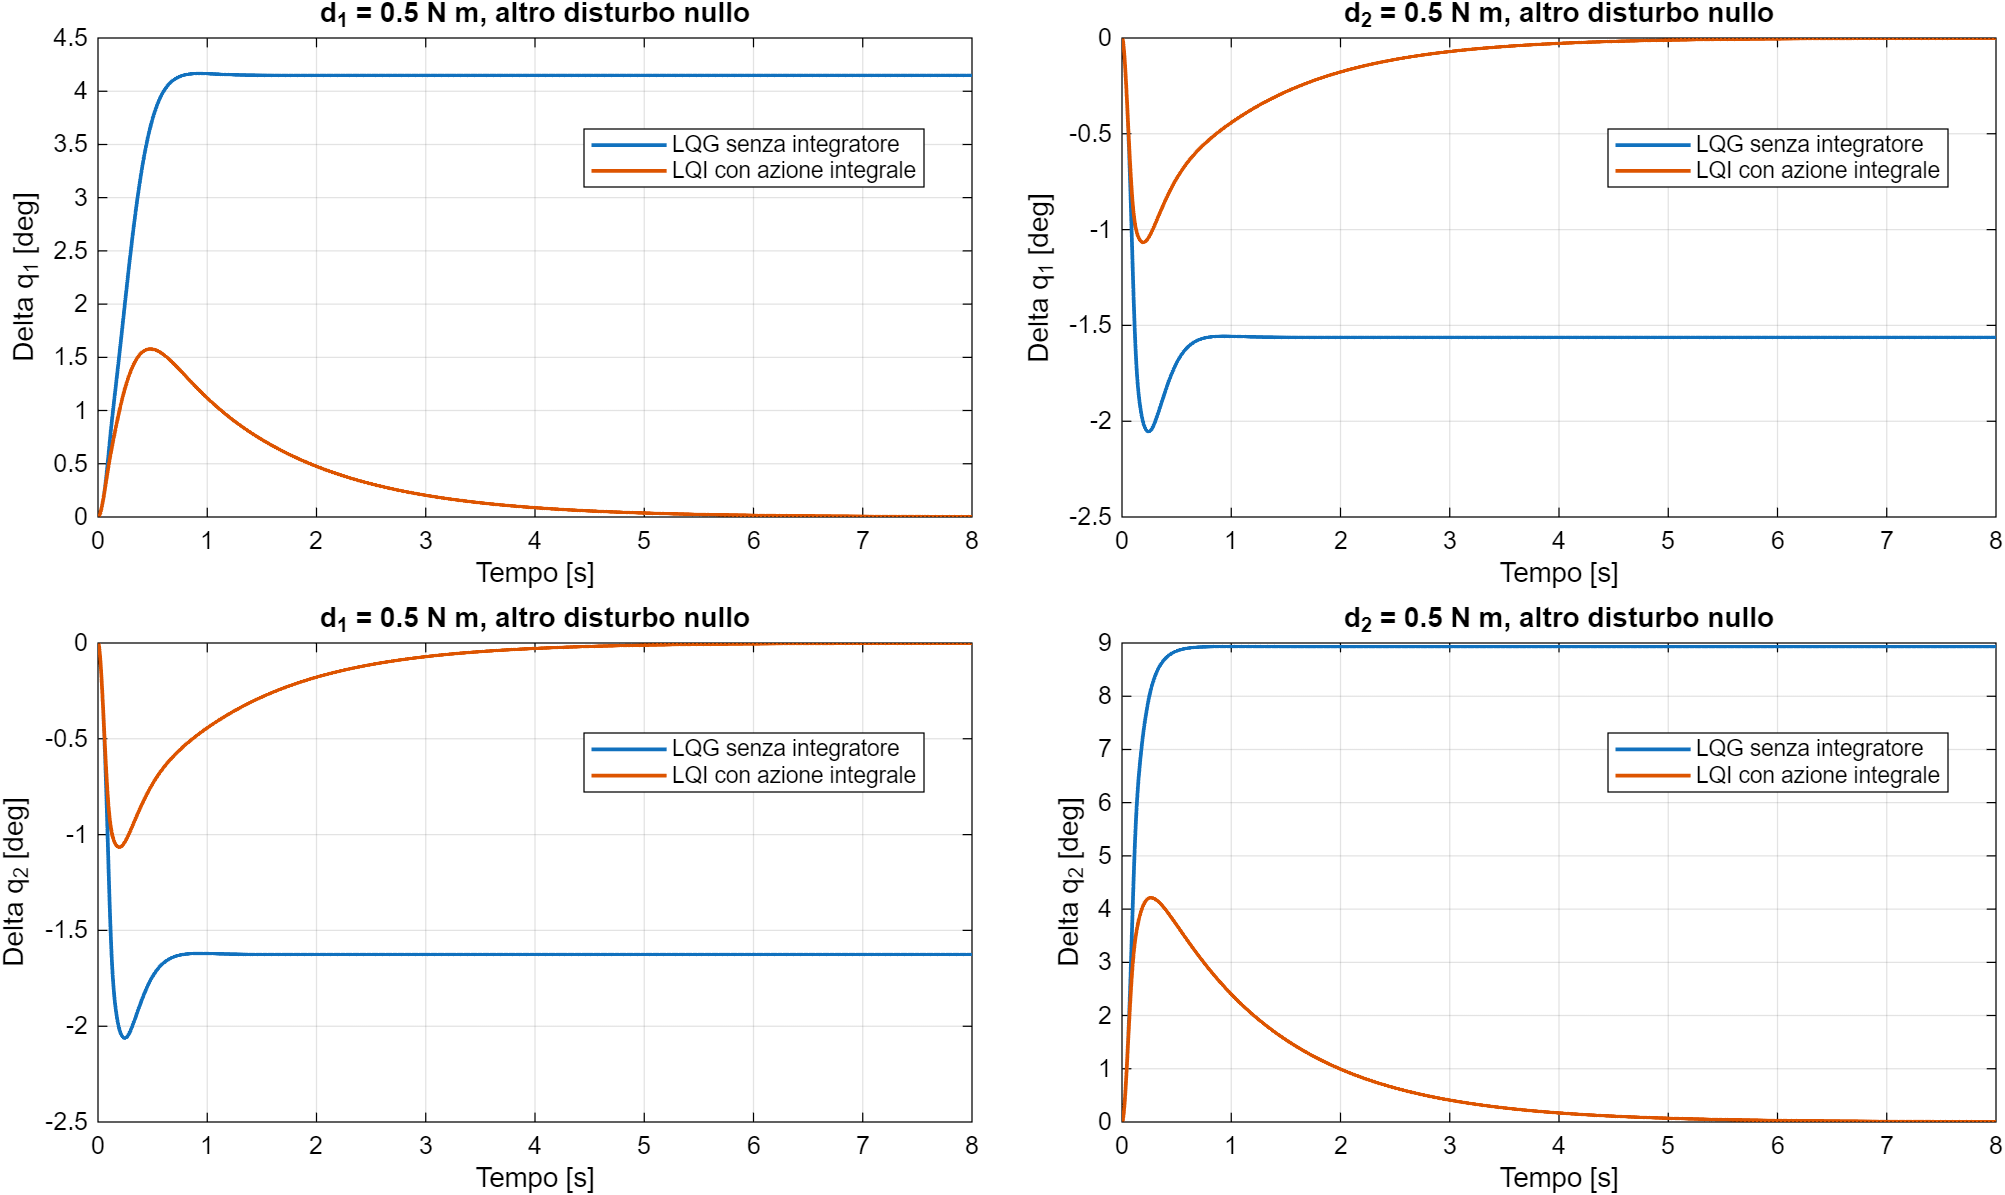
\includegraphics[width=0.86\textwidth]{figures/m7_lqg_lqi_constant_disturbance.png}
\caption{LQG senza integratore e LQI a stato vero, punto $(w_i,\rho_U)=(1,8)$, sotto le due coppie costanti da 0.5 N m. Tutti gli ingressi e gli stati iniziali sono identici; cambia l'architettura di feedback.}
\label{fig:lqi-disturbo}
\par\medskip
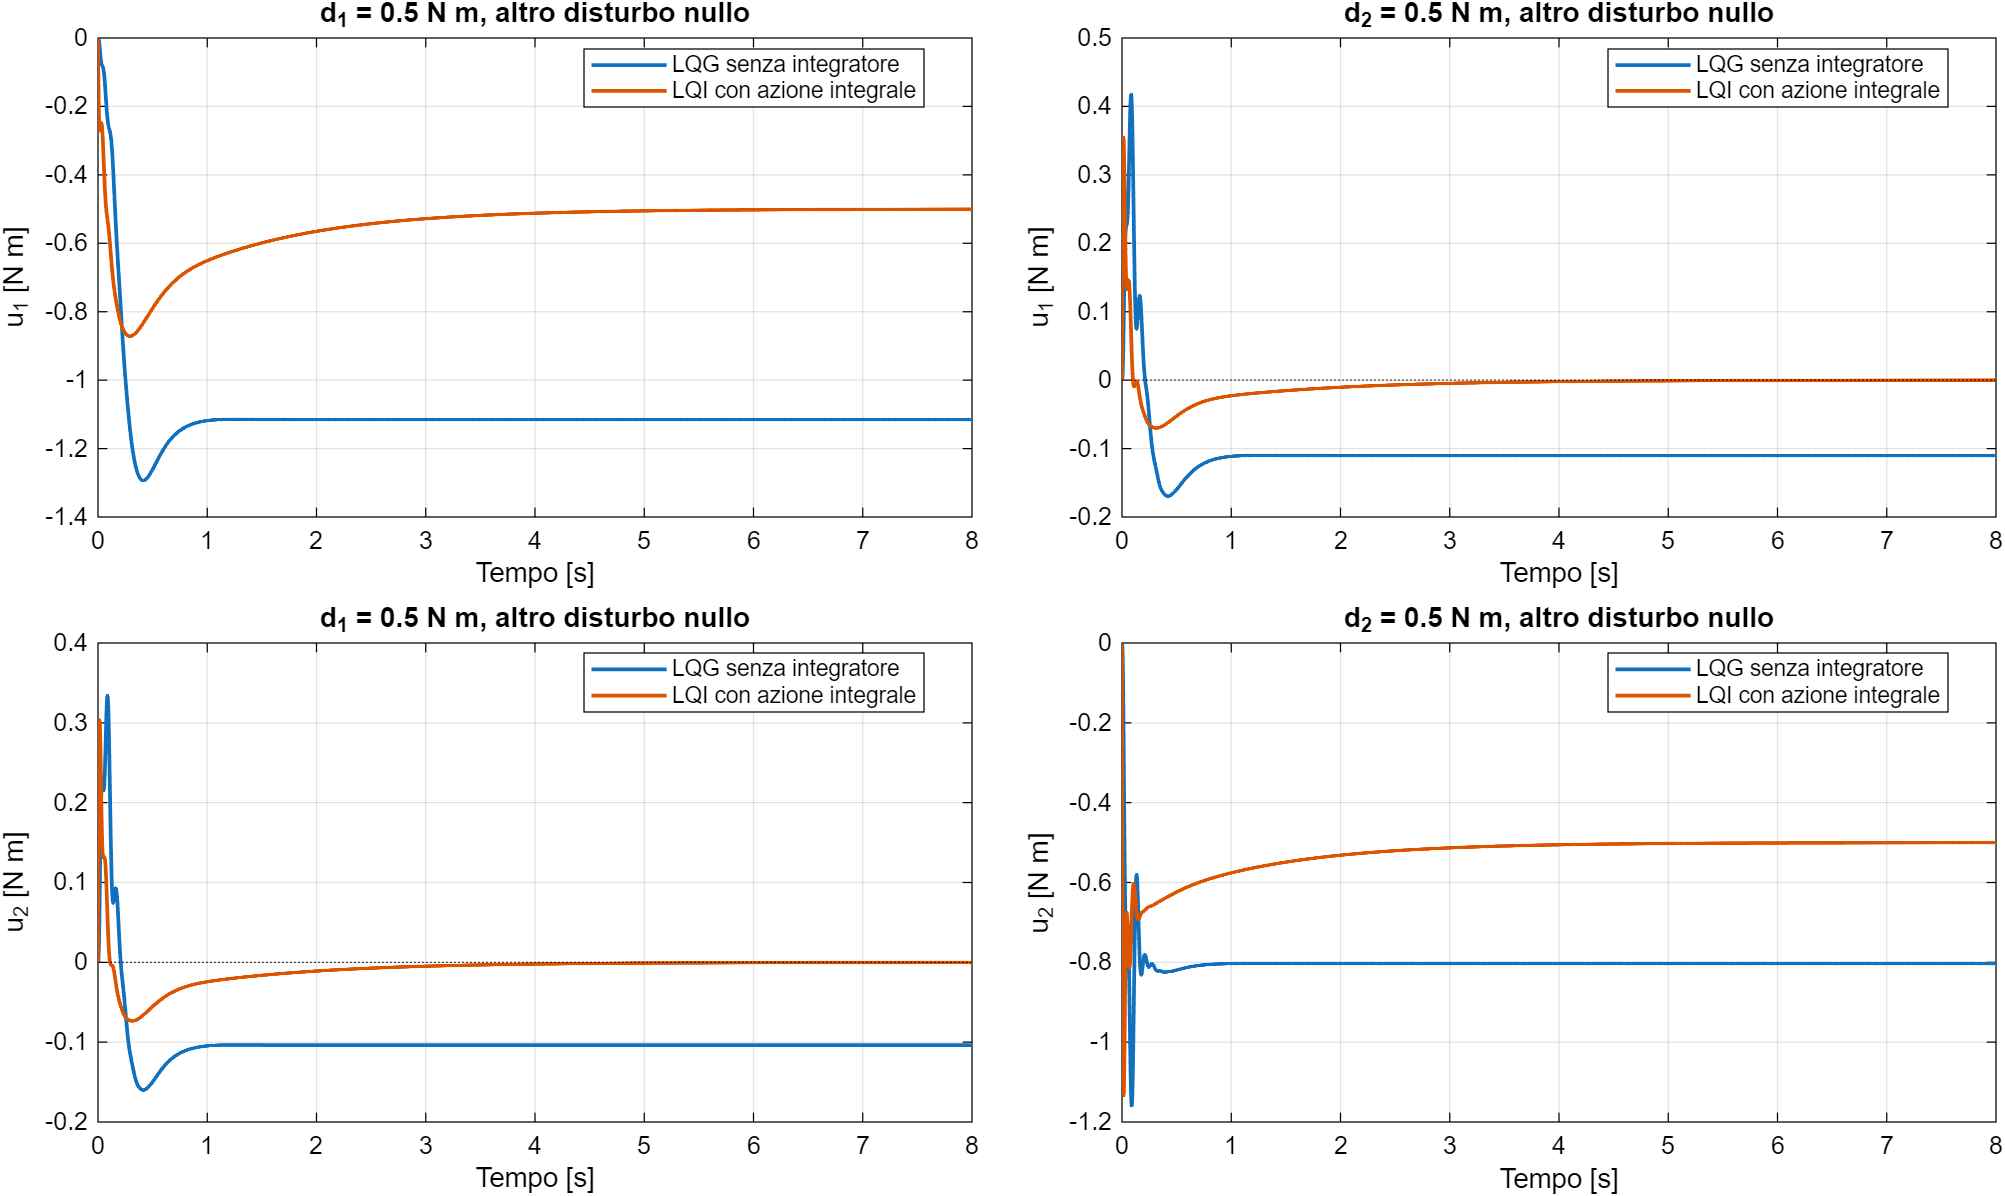
\includegraphics[width=0.86\textwidth]{figures/m7_lqg_lqi_disturbance_control.png}
\caption{Comandi degli stessi due esperimenti della Figura~\ref{fig:lqi-disturbo}. Non sono applicate saturazioni o compensazioni anti-windup.}
\label{fig:lqi-comando}
\end{figure}

\subsection{Perché lo studio non sostituisce il controllore nominale}
La Tabella~\ref{tab:lqi-tre-punti} conserva l'esito M7: tutti i punti sono
stabili e rigettano i disturbi costanti, ma i primi due non si assestano
entro 3 s e il terzo richiede $2.168$ s con overshoot $25.05\%$.
Il target M5 è $0.8$ s e $10\%$. Il punto intermedio usato nei grafici
ha overshoot $16.59\%$ e picco di tracking $7.805$ N m.
Il caso forte raggiunge $12.921$ N m: il superamento della scala
prestazionale di 12 N m non è una simulazione di saturazione hardware.

Se un attuatore reale saturasse, l'errore potrebbe continuare ad accumularsi
mentre il comando richiesto non è realizzabile: sarebbe necessaria una
strategia anti-windup, assente dal progetto. M7 resta dunque
\status{\MSevenStatus}, con \MSevenAdmissible\ punti conformi a tutti
i criteri. La reiezione dell'offset è un vantaggio reale, ma non basta
a sostituire M6 né a certificare robustezza.

\end{document}
